
\documentclass[12pt]{article}

% ── Packages ──────────────────────────────────────────────────────────────
\usepackage[T1]{fontenc}
\usepackage[utf8]{inputenc}
\usepackage{amsmath}
\usepackage{amssymb}
\usepackage{graphicx}
\usepackage{array}
\usepackage{url}
\usepackage{booktabs}
\usepackage{xcolor}
\usepackage{hyperref}
\usepackage[ruled,vlined,linesnumbered]{algorithm2e}
\usepackage{lineno}
\usepackage{microtype}
\usepackage[margin=1in]{geometry}
\emergencystretch=1em

% ── Graphics path ─────────────────────────────────────────────────────────
\graphicspath{{../figures/}}

\begin{document}

\title{CARL-WSN: Context-Aware Reinforcement Learning for Hybrid Routing in Heterogeneous IoT-Driven Wireless Sensor Networks}

\author{
Aymen Jaber Salman\thanks{Corresponding author. Email: aymen.j.salman@nahrainuniv.edu.iq} \and
Atheel Nowfal Alkhayyat\thanks{Email: atheel.n.al-khayyat@nahrainuniv.edu.iq} \and
Ruslan Saad Abdulrahman\thanks{Email: ruslan.s.al-nuaimi@nahrainuniv.edu.iq}
}
\date{Department of Computer Engineering, Al-Nahrain University, Baghdad, Iraq}

\maketitle

\begin{abstract}
Wireless Sensor Networks (WSNs) in IoT-driven smart cities carry heterogeneous
traffic with conflicting quality-of-service demands, yet no existing routing
protocol — including reinforcement learning (RL) approaches such as RLCR and
FQ-UCR, which apply Q-Learning within a single fixed paradigm — learns to
select between fundamentally different routing paradigms per packet, leaving
that choice urgency-blind. This paper introduces CARL-WSN, a Context-Aware RL
protocol that dynamically selects the routing paradigm — proactive, reactive,
or hybrid — per packet via tabular Q-Learning over a context vector of
urgency, residual energy, and link stability. A hard safety constraint forces
emergency traffic onto proactive routing regardless of policy, guaranteeing
sub-100~ms delivery. Evaluated in MATLAB against eight baselines — including
RPL, the IETF standard underlying the dominant real-world IoT mesh deployment
— over 720 runs on a common lossy-channel model with realistic control-plane
energy accounting, CARL-WSN attains a first-node-death lifetime statistically
tied with the strongest baseline and significantly ahead of most others;
achieves the second-lowest emergency latency of all nine protocols (24.7~ms,
23.8\% below AODV); and incurs overhead far below flooding- and table-based
protocols (0.52 vs.\ 14.91 for AODV), at a real, quantified delivery cost
(87.3\% PDR) arising from unconditional deferral of non-urgent traffic at
energy-critical nodes. These results show that learning which paradigm to
use, not merely optimizing within one, is an effective operating point for
heterogeneous, latency-critical IoT-WSN deployments.
\end{abstract}

\vspace{0.5em}
\noindent\textbf{Keywords:} Wireless sensor networks; Reinforcement learning; Q-Learning; Context-aware routing; Heterogeneous traffic; IoT; Energy-aware relay selection
\vspace{1em}

% ── SECTION I ─────────────────────────────────────────────────────────────────
\section{Introduction}
\label{sec:introduction}

The proliferation of Internet of Things (IoT) devices in smart city
infrastructure has transformed Wireless Sensor Networks (WSNs) from
single-application monitoring systems into multi-service platforms
that simultaneously carry traffic with fundamentally different
quality-of-service (QoS) requirements~\cite{akyildiz2002,zohrabi2024}.
A single WSN deployment may generate emergency alerts requiring
sub-100\,ms delivery, periodic telemetry tolerating delays of tens
of seconds, and event-driven uploads with best-effort requirements.
This traffic heterogeneity demands routing protocols that adapt their behaviour to the urgency class of individual packets — a capability absent from both classical and recent learning-based routing approaches. Even recent RL-based protocols such as RLCR~\cite{daanoune_intelligent_2026} and FQ-UCR~\cite{wang_fqucr_2025} apply Q-Learning only within a single fixed routing paradigm, leaving the choice between proactive, reactive, and hybrid routing itself unlearned and blind to packet urgency; this paper instead learns which paradigm to use, per packet, from a joint context of urgency, energy, and link stability.

Routing protocols for WSNs fall into three paradigms, each with
inherent trade-offs. Proactive protocols such as DSDV~\cite{perkins1994}
maintain routing tables continuously, delivering low latency at the
cost of high energy overhead from periodic broadcasts. Reactive protocols such as AODV~\cite{perkins1999} and DSR~\cite{johnson1996} discover routes on
demand,
conserving energy in low-traffic conditions but introducing
route-discovery delays of 20--100\,ms that violate emergency latency
constraints~\cite{selim_manet_2025}. Hybrid protocols such as
ZRP~\cite{haas2001} partition the network into zones and apply
different modes within and across boundaries, but use a fixed zone
radius that does not adapt to node energy state or traffic urgency.

Recent work has applied reinforcement learning (RL) to WSN routing
with promising results. Daanoune and Baghdad~\cite{daanoune_intelligent_2026}
proposed RLCR, a Q-Learning-based clustering and routing protocol
that optimises cluster head selection and inter-cluster forwarding
for energy efficiency. Wang and Duan~\cite{wang_fqucr_2025} proposed
FQ-UCR, combining fuzzy logic for unequal cluster formation with
Q-Learning for inter-cluster routing. While both protocols
demonstrate the potential of RL for adaptive WSN routing, they share
a fundamental limitation: routing decisions are made based on
network-level metrics (residual energy, distance to base station)
without any awareness of the application-level urgency class of
the packet being routed. An emergency alert and a routine temperature
reading receive identical routing treatment --- a systematic
inefficiency that leads to either wasted energy on low-urgency
traffic or dangerous delays on safety-critical packets.

A 2025 comprehensive survey by Khedr et al.~\cite{roberts2025}
explicitly identified dynamic application-context-based hybrid mode
switching as an open research direction in IoT-driven WSNs, noting
that reactive and hybrid context-aware approaches have received
significantly less attention than proactive ones. No published protocol closes this gap. This paper does so directly.

The main contributions of this paper are as follows:

\begin{itemize}
\item A formal Markov Decision Process (MDP) formulation for routing
paradigm selection in heterogeneous IoT-WSNs, with an 18-state
$\times$ 3-action state-action space derived from a three-dimensional
context vector comprising application urgency class~$U$, normalised
residual energy~$E_r$, and link stability score~$L_s$; of these 18
context states, 12 (corresponding to Class~B and Class~C) are
actively learned by the Q-learning agent, while the remaining 6
(Class~A) are governed by the hardcoded safety constraint and are
never updated by the learning process.

\item CARL-WSN, a Q-Learning-based routing protocol that learns the
optimal mapping from context states to routing paradigms (proactive,
reactive, or hybrid) through online interaction with the network
environment, using a class-dependent multi-objective reward function
that weights latency, overhead, and energy preservation according to
traffic priority. A safety constraint forces Class~A emergency
packets to proactive routing, guaranteeing sub-100\,ms delivery
regardless of the agent's learned policy.

\item An energy-aware relay selection mechanism combined with
critical-node packet deferral that extends network lifetime by
preferring high-residual-energy next-hop nodes and deferring
non-urgent packets when the transmitting node is near energy
depletion --- a context-aware lifetime extension capability that
only urgency-aware protocols can implement.

\item A comprehensive evaluation against eight baselines --- three classical protocols (AODV,
DSDV, ZRP), two domain-specific baselines (EH-Routing, MSLBA), two recent
RL-based protocols (RLCR, FQ-UCR), and the industry-standard RPL --- across four traffic scenarios and 20 independent
seeds (720 runs). Crucially, all nine protocols are re-implemented on a common
distance-dependent lossy-channel model with per-hop acknowledgement and retransmission, so that packet delivery, latency, and energy consumption emerge from identical
physical assumptions rather than from protocol-specific idealisations. Under this unified methodology,
CARL-WSN is statistically tied for the highest network lifetime, significantly leads
most baselines on half-node-death, and attains the second-lowest emergency-traffic
latency of all nine protocols, while incurring routing overhead far below the
flooding- and table-based protocols. These gains are obtained by trading a real,
quantified reduction in packet delivery, which we characterise explicitly.
\end{itemize}

The remainder of this paper is organised as follows.
Section~\ref{sec:related} reviews related work on hybrid, context-aware,
and RL-based routing in WSNs. Section~\ref{sec:model} presents the
system model. Section~\ref{sec:protocol} describes the CARL-WSN
protocol design, including the MDP formulation and Q-Learning
mechanism. Section~\ref{sec:simulation} presents the simulation setup.
Section~\ref{sec:results} presents and analyses the results.
Section~\ref{sec:discussion} discusses key findings, trade-offs, and
limitations. Section~\ref{sec:conclusion} concludes the paper.

% ── SECTION II ────────────────────────────────────────────────────────────────

\section{Related Work}
\label{sec:related}

\subsection{Proactive and Reactive Routing Protocols}

Routing protocols for WSNs have been extensively surveyed and
classified~\cite{akkaya2005}. Proactive protocols maintain routing
tables continuously through periodic broadcasts. DSDV~\cite{perkins1994}
established the foundational destination-sequenced distance-vector
approach, guaranteeing loop-free routes at all times.
OLSR~\cite{clausen2003} extended this paradigm through multipoint relay
selection, substantially reducing flooding overhead in dense networks.
While proactive protocols deliver consistently low latency by
eliminating route discovery delays, their continuous maintenance
overhead leads to significant energy waste on low-traffic
nodes~\cite{akkaya2005}.

Reactive protocols discover routes exclusively on demand.
AODV~\cite{perkins1999} pioneered this approach by initiating route
requests only when data must be transmitted, conserving energy in
sparse or low-traffic conditions. However, the route-discovery delay introduced by on-demand RREQ/RREP flooding
can make reactive protocols less suitable for the most latency-sensitive
traffic unless routes are cached and reused~\cite{selim_manet_2025}. A comparative analysis by
Nurul Hidayah et al.~\cite{nurul_hidayah_ahmad_zukri_comparative_2025}
confirmed that neither proactive nor reactive protocols alone achieve
optimal performance across varying network conditions, motivating the
need for adaptive hybrid approaches. Recent work~\cite{karthikeyan_optimizing_2025}
demonstrated that AODV, DSDV, and DSR all exhibit significant
performance degradation under heterogeneous traffic loads, highlighting
the fundamental limitation of single-mode routing for IoT-driven
smart city deployments.

\subsection{Hybrid Routing Protocols}

Hybrid protocols attempt to combine the latency advantages of
proactive routing with the energy efficiency of reactive routing.
ZRP~\cite{haas2001} pioneered zone-based hybrid routing by maintaining
proactive routes within a fixed-radius zone and using reactive
inter-zone routing for destinations beyond the zone boundary. While
ZRP reduces control overhead compared to purely proactive protocols,
its fixed zone radius is configured statically and does not adapt to
node energy state or traffic urgency.

Subsequent hybrid approaches incorporated additional optimisation
dimensions. Chaurasiya et al.~\cite{chaurasiya_energy-efficient_2023}
proposed a hybrid clustering technique for multilevel heterogeneous
IoT WSNs, combining cluster-based organisation with multi-hop routing
to reduce energy consumption. Lei~\cite{lei_energy-aware_2024}
proposed a hybrid energy-aware approach combining particle swarm
optimisation with fuzzy clustering for IoT routing, demonstrating
52\% energy reduction compared to DEEC, though at the cost of
requiring offline training data. Nadanam
et al.~\cite{nadanam_innovative_2026} recently proposed a
quantum-optimised hybrid routing framework achieving 30\% energy
reduction, though the computational complexity of quantum optimisation
makes it unsuitable for resource-constrained sensor hardware.

A common limitation across all these hybrid approaches is that mode
selection or routing decisions are made based on a single optimisation
objective --- typically energy or load --- without awareness of the
application-level urgency of the traffic being routed.

\subsection{Context-Aware Routing in IoT-WSNs}

Context-aware computing for IoT was formally defined by Perera
et al.~\cite{perera_context_2014}, who identified five contextual
dimensions --- identity, location, activity, time, and relations ---
as fundamental to intelligent IoT decision making. This foundational
work motivates the use of contextual information in routing decisions,
though the specific application to RL-based WSN hybrid routing mode
selection had not been addressed until the present work.

Context-aware routing has since been applied across several IoT and
WSN domains. Monteiro et al.~\cite{monteiro_context-aware_2019}
proposed context-aware network selection in heterogeneous wireless
networks, demonstrating that context-driven decisions outperform
static policies, but their work focused on network selection rather
than intra-WSN routing mode switching. Sithik and
Kumar~\cite{sithik_intelligent_2022} proposed a multi-context aware
parent selection scheme for the RPL protocol using grey set theory,
incorporating multiple contextual parameters into routing metric
computation. However, their approach targets RPL parent selection
exclusively and does not implement dynamic switching between
fundamentally different routing paradigms based on application urgency
class. Karagiannis et al.~\cite{karagiannis_context-aware_2023}
proposed context-aware routing for fog computing systems, reducing
latency by 23\% and hop count by 73\%, though their work operates at
the fog layer rather than the WSN sensor layer and does not model
heterogeneous traffic classes with conflicting QoS requirements. Hasan
et al.~\cite{hasan_context-aware_2025} proposed a context-aware trust
prediction framework for opportunistic IoT routing using Bayesian
inference, achieving 88.9\% delivery ratio, though the trust-based
context dimension differs fundamentally from the urgency-energy-stability
context vector proposed in CARL-WSN. Akpakwu et al.~\cite{akpakwu_cacc_2020} proposed a context-aware
congestion control scheme for CoAP/UDP IoT networks, applying context
sensing to transport-layer decisions rather than routing.

Smart city IoT routing has also received significant attention.
Karunkuzhali et al.~\cite{karunkuzhali_oqr-sc_2022,karunkuzhali_qos-aware_2024}
proposed QoS-aware routing frameworks for IoT-WSNs in smart cities,
demonstrating that multi-class service differentiation improves
network performance. However, none of these works implement dynamic
routing paradigm switching based on per-packet application urgency.
El-Fouly et al.~\cite{el-fouly_environment-aware_2023} proposed
environment-aware real-time routing for multi-sink WSNs in smart
cities, incorporating deadline constraints and link quality metrics.
This work shares the multi-sink topology with our prior
work~\cite{salman2023} and considers real-time delivery requirements. Smart city IoT routing has also been addressed by Hanif
et al.~\cite{hanif_opportunistically_2018} through opportunistic
IoT-WSN integration, Inga et al.~\cite{inga_novel_2021} through WSN
sizing and routing optimisation, and Ekler
et al.~\cite{ekler_energy_2022} through energy-aware IoT routing
algorithms. However, none of these works implement dynamic routing
paradigm switching based on per-packet application urgency, nor do they model heterogeneous application urgency classes or implement context-driven mode switching.

\subsection{Reinforcement Learning for WSN Routing}

The application of reinforcement learning to WSN routing has emerged
as one of the most active research frontiers in recent
years~\cite{priyadarshi_energy-efficient_2024,priyadarshi_ai-based_2025,yilmaz_sustainable_2025}.
RL-based protocols offer the ability to learn routing policies
through online interaction with the network environment, adapting
to changing conditions without requiring explicit models or
predefined rules.

Daanoune and Baghdad~\cite{daanoune_intelligent_2026} proposed RLCR, a
reinforcement learning-based clustering and routing protocol for
heterogeneous WSNs. RLCR uses Q-Learning in two phases: first for
cluster head (CH) selection based on residual energy, distance to the
base station, and node density; and second for inter-cluster multi-hop
routing where each CH learns the optimal next-hop CH toward the base
station. RLCR demonstrated significant lifetime improvements over
LEACH and DEEC variants. However, RLCR does not differentiate traffic
by application urgency class --- all packets receive identical
routing treatment regardless of whether they carry emergency alerts
or routine telemetry. Furthermore, RLCR's RL agent operates
exclusively within the clustering paradigm and does not consider
switching between fundamentally different routing modes.

Wang and Duan~\cite{wang_fqucr_2025} proposed FQ-UCR, a hybrid
approach combining fuzzy logic (FL) for unequal cluster head selection
with Q-Learning for inter-cluster routing. FQ-UCR addresses the
hotspot problem by forming smaller clusters near the base station
and larger clusters at greater distances, using a fuzzy inference
system to compute CH selection probability. The Q-Learning agent then
selects the optimal forwarding CH for inter-cluster data relay.
FQ-UCR demonstrated improved energy efficiency and lifetime compared
to EEUC and CHEF. Similar to RLCR, however, FQ-UCR does not model
heterogeneous traffic classes or adapt routing behaviour to
application urgency.

Sudha et al.~\cite{sudha_intelligent_2025} combined Q-Learning with
machine learning for cluster head selection and routing in 5G-enabled
WSNs, demonstrating improved throughput over LEACH, but without
considering per-packet application urgency as a routing criterion.
Saadallah and Alabady~\cite{saadallah_comprehensive_2024} identified
energy-efficient context-sensitive routing as an open challenge in
their comprehensive IoT routing study, while Kumar
et al.~\cite{kumar_exploring_2025} confirmed through bibliometric
analysis that application-context awareness remains an emerging
research gap in energy-efficient IoT-WSN routing.

Table~\ref{tab:comparison} summarises the key distinguishing features
of CARL-WSN compared to the most closely related works. CARL-WSN is
the only protocol that combines RL-based learning with per-packet
application urgency awareness for full routing paradigm switching.
Graph neural network (GNN)-based routing approaches, which learn
routing decisions from a graph representation of network topology,
represent a further class of AI-based routing not included in this
comparison: GNN methods typically require global or multi-hop
topology information as input and impose computational and memory
costs that are difficult to justify on resource-constrained WSN
nodes at the per-packet decision granularity this study targets,
making them a complementary rather than directly comparable
approach to the tabular, per-packet, locally-computed methods
considered here.

\begin{table}[!t]
\renewcommand{\arraystretch}{1.2}
\caption{Comparison of CARL-WSN with Related Routing Works}
\label{tab:comparison}
\centering
\resizebox{\textwidth}{!}{%
\begin{tabular}{lccccccc}
\hline
\textbf{Protocol} & \textbf{AI/ML} & \textbf{Context} & \textbf{Mode} &
\textbf{Traffic} & \textbf{Urgency} & \textbf{Energy-aware} & \textbf{Paradigm} \\
 & \textbf{method} & \textbf{dims} & \textbf{switching} &
\textbf{classes} & \textbf{aware} & \textbf{relay} & \textbf{switching} \\
\hline
RLCR~\cite{daanoune_intelligent_2026} & Q-Learning & 3 & CH selection & 1 & No & No & No \\
FQ-UCR~\cite{wang_fqucr_2025} & Fuzzy + Q-Learning & 3 & CH selection & 1 & No & No & No \\
Sithik \& Kumar~\cite{sithik_intelligent_2022} & Grey set theory & 2 & RPL parent & 1 & No & No & No \\
Karagiannis et al.~\cite{karagiannis_context-aware_2023} & None & 2 & Fog forwarding & 1 & No & No & No \\
Hasan et al.~\cite{hasan_context-aware_2025} & Bayesian & 1 (trust) & Route selection & 1 & No & No & No \\
ZRP~\cite{haas2001} & None & 1 (zone) & Hybrid fixed & 1 & No & No & No \\
\textbf{CARL-WSN (Ours)} & \textbf{Q-Learning} & \textbf{3} & \textbf{Per-packet RL} & \textbf{3} & \textbf{Yes} & \textbf{Yes} & \textbf{Yes} \\
\hline
\end{tabular}}
\end{table}

\subsection{Research Gaps}

The preceding review reveals five specific gaps that motivate CARL-WSN.
First, Khedr et al.~\cite{roberts2025} conducted the first
comprehensive survey of context-aware routing in IoT-driven WSNs and
explicitly identified dynamic application-context-based mode switching
as an open research direction, noting that reactive and hybrid
context-aware methods have received significantly less attention than
proactive approaches. Second, existing RL-based WSN routing protocols
(RLCR~\cite{daanoune_intelligent_2026},
FQ-UCR~\cite{wang_fqucr_2025}) apply Q-Learning within a single
routing paradigm (clustering) without awareness of application
urgency class --- the RL agent cannot distinguish between emergency
and routine traffic. Third, Chu et al.~\cite{chu_leach_2026}, Khanna
et al.~\cite{khanna_energy-efficient_2021}, and Prashanth
et al.~\cite{prashanth2023} all noted that routing adaptation in
heterogeneous WSNs remains dominated by single-objective optimisation
approaches that cannot simultaneously satisfy the conflicting
requirements of heterogeneous application traffic classes.
Fourth,no published protocol uses RL to learn
which routing paradigm (proactive, reactive, or hybrid) to use for
each packet based on a joint context vector of urgency, energy, and
link stability. Fifth, no RL-based WSN routing protocol incorporates
a safety constraint that guarantees latency bounds for critical
traffic regardless of the learned policy --- a requirement for
safety-critical IoT deployments.

% ── SECTION III ───────────────────────────────────────────────────────────────
\section{System Model}
\label{sec:model}

\subsection{Network Topology}

Consider a WSN comprising $N$ heterogeneous sensor nodes deployed
randomly over a square area of side length $A$\,m according to a
uniform distribution. Let $\mathcal{N} = \{1, 2, \ldots, N\}$ denote
the set of all nodes. A base station (BS) is located at the centre of
the deployment area, and a secondary sink node is positioned at the
right boundary, consistent with the multi-sink topology in our prior
work~\cite{salman2023}. Both the BS and sink are assumed to have
unconstrained energy. Each sensor node $i \in \mathcal{N}$ is
characterised by a fixed position $(p_i^x, p_i^y)$ and a
heterogeneous initial energy $E_0^i$ drawn from a uniform distribution
$E_0^i \sim \mathcal{U}(E_{\min}, E_{\max})$, reflecting the reality
of diverse sensor hardware in smart city deployments~\cite{salman2021}.

A node $i$ is considered alive if its residual energy $E_i(t) > 0$ at
simulation round $t$, and dead otherwise. Dead nodes neither transmit
nor receive. The network is considered operational as long as at least
10\% of nodes remain alive.

\subsection{Traffic Model}\label{sec:traffic_model}

Smart city IoT deployments generate heterogeneous application traffic
with fundamentally different QoS requirements. This paper models three
traffic classes simultaneously:

\begin{itemize}
\item \textbf{Class~A --- Emergency traffic:} Generated by
safety-critical sensors such as fire detectors, intrusion alarms, and
accident monitors. Modelled as a Poisson process with arrival rate
$\lambda_A$. Strict latency requirement: end-to-end delay must not
exceed 100\,ms.

\item \textbf{Class~B --- Periodic telemetry:} Generated by
environmental sensors reporting temperature, humidity, air quality,
and energy consumption. Modelled as a deterministic periodic process
with one packet per minute. Tolerates delays up to 30\,seconds.

\item \textbf{Class~C --- Event-driven uploads:} Generated by motion
detectors, occupancy sensors, and camera triggers. Modelled as a
Poisson process with arrival rate $\lambda_C$. Best-effort delivery
with no hard latency constraint.
\end{itemize}

Each packet carries a class tag $U \in \{A, B, C\}$ in its header,
which is read by the CARL-WSN context classifier at the transmitting
node before routing decisions are made.

\subsection{Channel and Energy Model}

Wireless communication is modelled using the first-order radio energy
model~\cite{heinzelman2000}, which captures the dominant sources of
energy consumption in sensor nodes: electronics and amplification.
The energy consumed by node $i$ to transmit an $L$-bit packet to a
receiver at distance $d$ is:

\begin{equation}
E_{tx}(L, d) = \begin{cases}
L \cdot E_{elec} + L \cdot \varepsilon_{fs} \cdot d^2 & d < d_0 \\
L \cdot E_{elec} + L \cdot \varepsilon_{mp} \cdot d^4 & d \geq d_0
\end{cases}
\label{eq:etx}
\end{equation}

where $d_0 = \sqrt{\varepsilon_{fs} / \varepsilon_{mp}} = 87.71$\,m
is the crossover distance between free-space and multipath propagation
models. The energy consumed to receive an $L$-bit packet is:

\begin{equation}
E_{rx}(L) = L \cdot E_{elec}
\label{eq:erx}
\end{equation}

The residual energy of node $i$ after a transmission round is:

\begin{equation}
E_i(t+1) = E_i(t) - E_{tx}(L, d) - E_{rx}(L)
\label{eq:eresidual}
\end{equation}

subject to $E_i(t) \geq 0$.

\subsection{Link Reliability and Retransmission Model}

Unlike idealised evaluations that assume guaranteed delivery, all
protocols in this study transmit over a distance-dependent lossy
channel, so that packet delivery is an emergent outcome rather than
an assumption. The probability that an $L$-bit frame is successfully
received over a link of length $d$ is modelled by a logistic
packet-reception-ratio (PRR) function in the transitional-region
form of Zuniga and Krishnamachari~\cite{zuniga2004}:

\begin{equation}
\mathrm{PRR}(d) = \frac{1}{1 + \exp\!\big(\alpha_{ch}\,(d - \beta_{ch})\big)}
\label{eq:prr}
\end{equation}

where $\beta_{ch} = 90$\,m is the midpoint distance at which the
reception probability falls to one half, and $\alpha_{ch} = 0.18$
controls the sharpness of the transitional region. Links shorter than
$\beta_{ch}$ are highly reliable, while reliability degrades steeply
beyond it.

Each hop employs a stop-and-wait automatic-repeat-request (ARQ)
scheme consistent with IEEE~802.15.4~\cite{ieee802154}: a frame is
retransmitted up to $R_{\max} = 3$ times, and the hop succeeds if any
attempt is acknowledged. A packet is delivered to the base station
only if \emph{every} hop on its multi-hop path succeeds within its
retransmission budget; otherwise it is counted as lost. Each
transmission attempt --- successful or not --- consumes the energy in
(\ref{eq:etx})--(\ref{eq:erx}), so retransmissions over marginal
links are charged their true energy cost. To ensure a fair,
paired comparison, the per-link, per-attempt channel outcomes are
generated from a common random-number stream keyed on the seed,
round, and link, so that every protocol experiences an identical
channel realisation for a given seed.

End-to-end latency is likewise emergent: the latency of a delivered
packet is the sum over its hops of the per-hop transmission and
processing time plus the timeout penalty of any failed attempts,
rather than a fixed per-mode constant.

\subsection{Link Stability Model}

To capture dynamic link quality variations, CARL-WSN maintains a
per-node link stability score $L_s^i(t) \in [0, 1]$, computed as an
Exponential Weighted Moving Average (EWMA) of the ACK success history
over a sliding window of $W$ most recent transmissions:

\begin{equation}
L_s^i(t) = \sum_{k=0}^{W-1} w_k \cdot a_k^i
\label{eq:ls}
\end{equation}

where $a_k^i \in \{0, 1\}$ is the ACK outcome of the $k$-th most
recent transmission from node $i$, and
$w_k = \alpha_{\text{ewma}}(1 - \alpha_{\text{ewma}})^k / Z$ are normalised exponentially decaying
weights with smoothing factor $\alpha_{\text{ewma}} = 0.5$ and normalisation
constant $Z = \sum_{k=0}^{W-1}(1 - \alpha_{\text{ewma}})^k$, computed over a window
of $W = 30$ recent transmissions. These values follow the WMEWMA
link estimator of Woo and Culler~\cite{woo2003}. The score is
updated online from the real per-hop acknowledgement outcomes
produced by the ARQ mechanism of Section~\ref{sec:model}.

\subsection{Energy-Aware Relay Selection Model}

CARL-WSN introduces an energy-aware relay selection mechanism that
extends network lifetime by preferring next-hop nodes with higher
residual energy. When forwarding a packet, node $i$ selects the
next-hop relay $j^*$ from its set of alive neighbours
$\mathcal{N}_i = \{j : d_{ij} \leq R_{tx}, E_j(t) > 0\}$ by
maximising a composite score:

\begin{equation}
j^* = \arg\max_{j \in \mathcal{N}_i} \left[
  \left( w_p \cdot \frac{d_{iBS} - d_{jBS}}{d_{iBS}} +
  w_e \cdot \frac{E_j(t)}{E_0^j} \right) \cdot \mathrm{PRR}(d_{ij})
\right]
\label{eq:relay}
\end{equation}

where $d_{iBS}$ and $d_{jBS}$ are the distances from nodes $i$ and
$j$ to the base station respectively, $w_p = 0.4$ is the progress
weight, and $w_e = 0.6$ is the energy weight. The first term
encourages geographic progress toward the BS, while the second term
favours relays with higher residual energy ratios, distributing the
forwarding load away from energy-depleted nodes. The composite score
is further weighted by the link reliability $\mathrm{PRR}(d_{ij})$
from~(\ref{eq:prr}), so that the relay metric prefers next hops that
are simultaneously closer to the BS, higher in energy, and reliably
reachable. Only candidates with positive progress
($d_{jBS} < d_{iBS}$) are considered, ensuring packets always advance
toward the BS.

\subsection{Critical-Node Packet Deferral}

When a node's residual energy ratio falls below a critical threshold
$E_r^i < T_{defer}$, CARL-WSN defers transmission of non-urgent
packets (Class~B and Class~C) to preserve the node's remaining
energy. Because energy in this model is strictly non-increasing
(Eq.~\ref{eq:eresidual} admits no harvesting or recovery term), a
node that has crossed $T_{defer}$ can never subsequently return above
it: its energy state can only remain at or fall further below the
threshold for the remainder of its operational life. Consequently,
once triggered, deferral is unconditional and permanent for that
node's non-urgent traffic --- there is no physically meaningful
condition under which a deferred packet could later be transmitted,
since the ``improved conditions'' that would justify release from
deferral cannot occur. This design directly follows from the
reviewer-raised requirement that deferred traffic be either
transmitted once conditions improve or treated as expired: since the
former is provably impossible under the non-increasing energy model,
every deferred packet's outcome is equivalent to immediate expiry,
and is accounted as such rather than through an artificial bounded
retry mechanism. Deferred packets incur only a minimal listening
energy cost of $0.1 \cdot L \cdot E_{elec}$ and are counted as
offered-but-not-delivered, so deferral trades packet delivery for
extended lifetime. The operating point used in this paper,
$T_{defer} = 0.05$, is selected from the sensitivity analysis in
Section~\ref{sec:sensitivity} to retain the lifetime gain at a
modest delivery cost. Class~A emergency packets are never deferred
regardless of node energy state --- the safety constraint takes
absolute priority. This deferral mechanism is a unique capability of
urgency-aware protocols: baseline protocols that do not distinguish
traffic classes cannot selectively defer low-priority traffic to
extend node lifetime.

\subsection{Performance Metrics}

Eight metrics are used to evaluate protocol performance:

\textbf{Network lifetime:} The First Node Death round
$r_{FND} = \min\{t : \exists\, i,\, E_i(t) = 0\}$ and the Half
Node Death round $r_{HND} = \min\{t : |\{i : E_i(t) = 0\}|
\geq N/2\}$.

\textbf{Packet Delivery Ratio:}
\begin{equation}
PDR = \frac{D_{delivered}}{D_{total}}
\label{eq:pdr}
\end{equation}

\textbf{Energy balance} (Gini coefficient):
\begin{equation}
G = \frac{2 \sum_{i=1}^{N} i \cdot c_i}{N \sum_{i=1}^{N} c_i}
  - \frac{N+1}{N}
\label{eq:gini}
\end{equation}

where $c_i$ is the energy consumed by node $i$, sorted in ascending
order ($c_1 \leq c_2 \leq \cdots \leq c_N$). A lower $G$ indicates
more uniform energy consumption.

\textbf{Routing overhead:}
\begin{equation}
\Omega = \frac{C_{ctrl}}{D_{total}}
\label{eq:overhead}
\end{equation}

where $C_{ctrl}$ is the total number of routing control packets
generated during the simulation.

\textbf{Additional metrics:} Mean Class~A latency, average energy
consumed per round, and network throughput (packets delivered per
round).

% ── SECTION IV ────────────────────────────────────────────────────────────────
\section{CARL-WSN Protocol Design}
\label{sec:protocol}

\subsection{Design Motivation}

Existing RL-based WSN routing protocols apply Q-Learning within a
single routing paradigm. RLCR~\cite{daanoune_intelligent_2026} uses
Q-Learning for cluster head selection and inter-cluster forwarding
--- both decisions operate within the clustering paradigm.
FQ-UCR~\cite{wang_fqucr_2025} similarly applies Q-Learning only to
select the next forwarding cluster head. In both protocols, the
fundamental routing mechanism (clustering with multi-hop inter-cluster
relay) never changes regardless of traffic urgency.

CARL-WSN addresses a categorically different problem: \emph{which
routing paradigm should be used for each packet?} The RL agent learns
to select between proactive, reactive, and hybrid routing --- three
fundamentally different mechanisms with distinct latency, overhead,
and energy characteristics --- based on a per-packet context vector
that includes application urgency class. This is routing paradigm
switching, not routing optimisation within a fixed paradigm.

\subsection{The Context Vector}

For each packet to be transmitted by node $i$ of class $U$, the
context vector $\mathbf{C}_i = (U, E_r^i, L_s^i)$ is computed, where:

\begin{itemize}
\item $U \in \{A, B, C\}$ is the urgency class read directly from the
packet header. Zero additional computation is required.

\item $E_r^i = E_i(t) / E_0^i \in [0, 1]$ is the normalised residual
energy ratio. $E_r^i = 1$ indicates full energy; $E_r^i \to 0$
indicates near-depletion.

\item $L_s^i \in [0, 1]$ is the link stability score computed
using~(\ref{eq:ls}).
\end{itemize}

\subsection{MDP Formulation}

The routing paradigm selection problem is formulated as a Markov
Decision Process $(\mathcal{S}, \mathcal{A}, R, \gamma)$ where each
packet transmission constitutes one decision step.

\subsubsection{State Space}\label{sec:state_space}

The continuous context vector is discretised into a finite state space
suitable for tabular Q-Learning:

\begin{itemize}
\item Urgency class $U$: 3 values --- $A$ (emergency), $B$
(telemetry), $C$ (event-driven).

\item Residual energy level: 3 levels --- low ($E_r^i < 0.3$),
mid ($0.3 \leq E_r^i < 0.7$), high ($E_r^i \geq 0.7$).

\item Link stability level: 2 levels --- unstable ($L_s^i < 0.7$),
stable ($L_s^i \geq 0.7$).
\end{itemize}

The total state space is $|\mathcal{S}| = 3 \times 3 \times 2 = 18$
states. Each state is encoded as a linear index:

\begin{equation}
s = (U_{num} - 1) \times 6 + (E_{level} - 1) \times 2 + L_{level}
\label{eq:state}
\end{equation}

where $U_{num} \in \{1, 2, 3\}$, $E_{level} \in \{1, 2, 3\}$, and
$L_{level} \in \{1, 2\}$. Table~\ref{tab:states} enumerates all 18
states with their physical interpretations.

\begin{table}[!t]
\renewcommand{\arraystretch}{1.1}
\caption{CARL-WSN State Space: All 18 States}
\label{tab:states}
\centering
\resizebox{\textwidth}{!}{%
\begin{tabular}{clccc}
\hline
\textbf{State} & \textbf{Real-world meaning} & $U$ & $E_r$ \textbf{level} & $L_s$ \textbf{level} \\
\hline
1--2   & Emergency, low energy, unstable/stable link   & A & low  & unstable/stable \\
3--4   & Emergency, moderate energy, unstable/stable    & A & mid  & unstable/stable \\
5--6   & Emergency, healthy node, unstable/stable       & A & high & unstable/stable \\
7--8   & Telemetry, low energy, unstable/stable         & B & low  & unstable/stable \\
9--10  & Telemetry, moderate energy, unstable/stable    & B & mid  & unstable/stable \\
11--12 & Telemetry, healthy node, unstable/stable       & B & high & unstable/stable \\
13--14 & Best-effort, low energy, unstable/stable       & C & low  & unstable/stable \\
15--16 & Best-effort, moderate energy, unstable/stable  & C & mid  & unstable/stable \\
17--18 & Best-effort, healthy node, unstable/stable     & C & high & unstable/stable \\
\hline
\end{tabular}}
\end{table}

\subsubsection{Action Space}

The agent selects one of three routing paradigms per packet:

\begin{equation}
\mathcal{A} = \{\text{proactive},\; \text{reactive},\; \text{hybrid}\}
\label{eq:actions}
\end{equation}

The Q-table has dimensions $18 \times 3 = 54$ entries, requiring
only $54 \times 4 = 216$ bytes of storage in single-precision
floating point --- deployable on any sensor platform with at least
1\,KB of RAM.

\subsubsection{Reward Function}

After selecting action $a$ in state $s$, the agent observes the
routing outcome and receives a class-dependent multi-objective reward:

\begin{equation}
R(s, a) = w_1^U \cdot R_{lat} + w_2^U \cdot R_{oh} + w_3^U \cdot R_{en}
\label{eq:reward}
\end{equation}

where the three reward components are:

\begin{equation}
R_{lat} = \begin{cases}
-1 & \text{if } U = A \text{ and } \ell > 100\,\text{ms} \\
1 - \ell / \ell_{\max}^U & \text{otherwise}
\end{cases}
\label{eq:rlat}
\end{equation}

\begin{equation}
R_{oh} = 1 - \min\!\left(\frac{c_{ctrl}}{n_{nb} \cdot 0.20},\; 1\right)
\label{eq:roh}
\end{equation}

\begin{equation}
R_{en} = \min\!\left(\frac{E_r^{after}}{E_r^{before}},\; 1\right)
\label{eq:ren}
\end{equation}

Here $\ell$ is the observed end-to-end latency, $\ell_{\max}^U$ is
the class-specific latency tolerance (100\,ms for Class~A, 30\,s for
Class~B, $\infty$ for Class~C), $c_{ctrl}$ is the number of control
packets generated, $n_{nb}$ is the neighbour count, and $E_r^{before}$
and $E_r^{after}$ are the residual energy ratios before and after
transmission.

The class-dependent weight vectors are:

\begin{equation}
(w_1^U, w_2^U, w_3^U) = \begin{cases}
(0.7,\; 0.15,\; 0.15) & U = A \text{ (latency dominates)} \\
(0.2,\; 0.3,\;\; 0.5)  & U = B \text{ (energy dominates)} \\
(0.1,\; 0.3,\;\; 0.6)  & U = C \text{ (energy dominates)}
\end{cases}
\label{eq:weights}
\end{equation}

This formulation ensures that the RL agent learns different routing
preferences for different traffic classes: Class~A packets are
penalised heavily for latency violations, while Class~B and Class~C
packets are rewarded primarily for energy preservation. The weight
vectors encode the fundamental QoS distinction between emergency and
non-emergency IoT traffic.

\subsubsection{Q-Learning Update Rule}

The Q-table is updated after each packet transmission using the
standard Q-Learning rule:

\begin{equation}
Q(s, a) \leftarrow Q(s, a) + \alpha \left[
  R(s, a) + \gamma \max_{a'} Q(s', a') - Q(s, a)
\right]
\label{eq:qupdate}
\end{equation}

where $\alpha = 0.1$ is the learning rate, $\gamma = 0.9$ is the
discount factor, $s'$ is the next state observed after packet
delivery, and $\max_{a'} Q(s', a')$ is the maximum expected future
reward from the next state.

Action selection follows an $\varepsilon$-greedy policy:

\begin{equation}
a = \begin{cases}
\text{random action from } \mathcal{A} & \text{with probability } \varepsilon \\
\arg\max_a Q(s, a) & \text{with probability } 1 - \varepsilon
\end{cases}
\label{eq:egreedy}
\end{equation}

The exploration rate decays exponentially:

\begin{equation}
\varepsilon_{t+1} = \max(\varepsilon_t \cdot \delta,\; \varepsilon_{\min})
\label{eq:epsdecay}
\end{equation}

with initial $\varepsilon_0 = 0.1$, decay factor $\delta = 0.998$, and minimum $\varepsilon_{\min} = 0.01$. This schedule
ensures sufficient exploration in early rounds while converging to a near-greedy exploitation
policy within approximately 1345 rounds.

\subsection{Safety Constraint}

A critical design requirement for safety-critical IoT deployments is
that emergency traffic must \emph{never} be delayed by route
discovery, regardless of what the RL agent has learned. CARL-WSN
enforces this through a hard constraint that overrides the agent's
policy:

\begin{equation}
\text{If } U = A: \quad a = \text{proactive} \quad \text{(unconditional)}
\label{eq:safety}
\end{equation}

This constraint is applied \emph{before} the $\varepsilon$-greedy
selection in~(\ref{eq:egreedy}), ensuring that Class~A packets are
always routed via proactive mode with pre-built routing tables,
guaranteeing sub-100\,ms delivery at all times. The Q-table entries
for states 1--6 (all Class~A states) are never updated by the agent
--- proactive routing for emergencies is a design invariant, not a
learned behaviour.

This separation between learned policy (Class~B and~C) and hardcoded
safety guarantee (Class~A) is a distinguishing feature of CARL-WSN.
Neither RLCR~\cite{daanoune_intelligent_2026} nor
FQ-UCR~\cite{wang_fqucr_2025} implements traffic-class-specific
safety constraints, because neither protocol differentiates traffic
by urgency class.

\subsection{Routing Modes}

The three routing paradigms available to the RL agent are:

\subsubsection{Proactive Mode}
Inspired by DSDV~\cite{perkins1994}, proactive mode maintains routing
tables through periodic broadcasts every round. When a packet requires
transmission, the next hop toward the BS is selected using the
energy-aware relay selection mechanism defined in~(\ref{eq:relay}),
combining geographic progress with residual energy preference.
The energy overhead includes both data transmission cost and a table
maintenance overhead of 10\% of the data packet energy per round.
This mode is mandatory for Class~A emergency traffic and is also
selected by the RL agent when link instability makes reactive
route discovery unreliable.

\subsubsection{Reactive Mode}
Inspired by AODV~\cite{perkins1999}, reactive mode initiates route
discovery only when a packet needs to be sent. A Route Request (RREQ)
is flooded to neighbours within transmission range, and a Route Reply
(RREP) is returned along the reverse path with energy-aware relay
selection applied at each hop. This
eliminates periodic broadcast overhead at the cost of an on-demand
route-discovery delay on a cache miss. Discovered routes are cached and
reused while valid, so the discovery cost is amortised over subsequent
packets to the same destination; the per-packet latency is therefore emergent
--- the sum of per-hop transmission times plus the discovery round-trip on the
fraction of packets that miss the cache --- rather than a fixed per-mode
constant.
The RL agent learns to select reactive mode primarily for Class~B and
Class~C traffic on healthy nodes with stable links, where the energy
saving from avoiding table maintenance outweighs the latency cost.

\subsubsection{Hybrid Mode}
Extending ZRP~\cite{haas2001}, hybrid mode maintains proactive routes
within a dynamically-sized zone and uses reactive inter-zone routing
beyond the zone boundary. The proactive zone radius adapts based on
the node's residual energy ratio:

\begin{equation}
r_{zone}^i = \begin{cases}
120\,\text{m} & E_r^i \geq 0.6 \text{ (healthy)} \\
80\,\text{m}  & 0.3 \leq E_r^i < 0.6 \text{ (moderate)} \\
40\,\text{m}  & E_r^i < 0.3 \text{ (critical)}
\end{cases}
\label{eq:zone}
\end{equation}

The RL agent learns to select hybrid mode primarily for energy-critical
nodes carrying non-emergency traffic, where the reduced zone radius limits
broadcast overhead while maintaining route availability within the immediate
neighbourhood. Note that the $0.6$ energy cut-off defining the healthy zone
radius here is distinct from the $0.7$ residual-energy boundary used to
discretise the state space in Section~\ref{sec:state_space}: the former tunes
the continuous zone-radius response of the hybrid mode, whereas the latter sets
the coarse energy level fed to the tabular Q-agent. The two thresholds control
different mechanisms and are therefore set independently.

Mode selection governs only how a packet's source node discovers or
maintains next-hop information (continuously, on demand, or within
a bounded zone); once a next hop is determined, forwarding proceeds
identically for every packet via the shared relay-selection
mechanism in~(\ref{eq:relay}), regardless of mode. Relay nodes
therefore require no mode of their own, permitting different
packets to use different modes concurrently without inconsistency.

\subsection{Complete Per-Packet Routing Procedure}

Algorithm~\ref{alg:carlwsn} presents the complete per-packet routing
procedure, integrating the context vector computation, safety
constraint, $\varepsilon$-greedy action selection, energy-aware
routing, packet deferral, and Q-table update.

\begin{algorithm}[!t]
\caption{CARL-WSN Per-Packet Routing with Q-Learning}
\label{alg:carlwsn}
\SetAlgoLined
\KwIn{Packet $p$ with class $U$, node $i$, network state $\mathcal{N}$, Q-table $Q$, exploration rate $\varepsilon$}
\KwOut{Updated network state, updated Q-table}

\tcp{Step 1: Compute context vector}
$U \gets \textsc{ReadClassTag}(p)$\;
$E_r^i \gets E_i(t) / E_0^i$\;
$L_s^i \gets \sum_{k=0}^{W-1} w_k \cdot a_k^i$\;
$s \gets \textsc{StateIndex}(U, E_r^i, L_s^i)$\;

\eIf{$U = A$}{
  \tcp{Step 2: Safety constraint --- emergency traffic bypasses learning}
  $a \gets$ proactive\;
}{
  \tcp{Step 3: Unconditional critical-node deferral}
\If{$E_r^i < T_{\text{defer}}$ \textbf{and} $U \in \{B, C\}$}{
    Defer packet permanently (minimal listening energy cost)\;
    \Return\;
}
  \tcp{Step 4: $\varepsilon$-greedy action selection}
  \eIf{$\mathrm{rand}() < \varepsilon$}{
    $a \gets$ random action from $\mathcal{A}$\;
  }{
    $a \gets \arg\max_{a'} Q(s, a')$\;
  }
}

\tcp{Step 5: Route with energy-aware relay}
$j^* \gets \arg\max_{j \in \mathcal{N}_i} \left[ \left( 0.4 \cdot \mathrm{progress}(j) + 0.6 \cdot E_r^j \right) \cdot \mathrm{PRR}(d_{ij}) \right]$\;
Route packet via mode $a$ using relay $j^*$\;

\tcp{Step 6: Observe outcome and compute reward}
$R \gets w_1^U \cdot R_{lat} + w_2^U \cdot R_{oh} + w_3^U \cdot R_{en}$\;
$s' \gets \textsc{StateIndex}(U, E_r^{i,new}, L_s^{i,new})$\;

\tcp{Step 7: Q-table update (skip for Class A)}
\If{$U \neq A$}{
  $Q(s, a) \gets Q(s, a) + \alpha [R + \gamma \max_{a'} Q(s', a') - Q(s, a)]$\;
}

$\varepsilon \gets \max(\varepsilon \cdot \delta, \varepsilon_{\min})$\;
\end{algorithm}

\subsection{Overhead Analysis}

The per-packet control overhead $\omega$ of CARL-WSN adapts to the
selected mode:

\begin{equation}
\omega = \begin{cases}
n_{nb} \cdot 0.08 & \text{proactive (Class~A)} \\
n_{nb} \cdot 0.05 & \text{reactive (Class~B/C)} \\
n_{nb} \cdot 0.06 & \text{hybrid}
\end{cases}
\label{eq:overhead_modes}
\end{equation}

where $n_{nb}$ is the number of one-hop neighbours within 100\,m
range. By selecting reactive mode for the majority of Class~B and~C
traffic when conditions permit, CARL-WSN avoids the continuous
broadcast overhead that makes purely proactive protocols
(DSDV: $\omega = n_{nb} \cdot 0.20$ per packet) energy-intensive.

\subsection{Computational Complexity}

The context classifier operates in $O(1)$ time per packet: urgency
class $U$ is read from the packet header in constant time, $E_r^i$
is a single division operation, $L_s^i$ is a fixed-length dot product
over $W = 30$ values, state indexing requires three integer
operations, and the Q-table lookup is a single array access. The Q-Learning update in~(\ref{eq:qupdate}) requires one multiplication,
one addition, and one max operation over 3 values --- all $O(1)$.
The total per-packet computational overhead is an analytical estimate
of under 0.1\,ms, based on operation count on a modern
floating-point-capable sensor processor; on microcontrollers lacking
a hardware floating-point unit, the constituent floating-point
operations would require software emulation, increasing this
estimate substantially, though the total is still expected to remain
small relative to radio transmission time. Fixed-point arithmetic is
a practical mitigation for FPU-less platforms that we did not
evaluate in this study. The memory footprint comprises the Q-table
(216~bytes), the ACK history buffer (80~bytes), the state index
computation variables (12~bytes), and a neighbour-state table
required for the energy-aware relay selection in~(\ref{eq:relay}),
which was omitted from an earlier accounting. Each entry stores a
neighbour identifier, a quantised residual-energy estimate, and a
distance-to-base-station value (4~bytes per neighbour); measured
directly across all 100 nodes and 20 seeds of this study's
deployment, the mean neighbour count is 48.0 (std.\ 14.0, range
13--85), giving a neighbour-state table of 192~bytes on average and
340~bytes in the worst observed case. The complete memory footprint
is therefore 500~bytes on average (648~bytes worst-case), still
comfortably deployable on TelosB (10\,KB RAM), MicaZ (4\,KB RAM),
and Arduino-class devices without modification.

\subsection{Rule-Based Ablation: Isolating the Value of Learning}
\label{sec:rule_ablation}

To test whether the learned Q-table earns its complexity over a
non-learned alternative, we construct CARL-Rule: a fixed-rule variant
that is architecturally identical to CARL-WSN --- the same safety
constraint, the same critical-node deferral mechanism, the same
energy-aware relay selection and channel model --- but replaces only
the learned mode-selection step (Section~4.3.4) with a static,
three-branch rule:
\begin{equation}
mode =
\begin{cases}
\text{proactive} & \text{if } L_s^i < T_L \\
\text{hybrid} & \text{else if } E_r^i < T_E \\
\text{reactive} & \text{otherwise}
\end{cases}
\label{eq:rule_ablation}
\end{equation}
This rule is derived directly from CARL-WSN's own stated design
rationale in Sections~4.5.1--4.5.3 --- proactive mode is selected
``when link instability makes reactive route discovery unreliable''
(Section~4.5.1), hybrid mode is selected ``primarily for
energy-critical nodes'' (Section~4.5.3), and reactive mode is
selected ``primarily... on healthy nodes with stable links''
(Section~4.5.2) --- and not from the agent's learned policy
(Fig.~\ref{fig:policy}) or Q-values (Fig.~\ref{fig:qvalues}), so that
the comparison is not circular. $T_L$ and $T_E$ retain the same
values and roles as in the state discretisation (Table~2).
CARL-Rule is evaluated under the identical experimental protocol as
the nine main protocols, across all four traffic scenarios and 20
seeds.

% ── SECTION V ─────────────────────────────────────────────────────────────────
\section{Simulation Setup}
\label{sec:simulation}

\subsection{Network Model}

The simulation models a smart city IoT-WSN deployment comprising
$N = 100$ heterogeneous sensor nodes randomly distributed over a
$200 \times 200$\,m$^2$ area using a uniform random distribution.
A base station is positioned at the centre of the deployment area
at coordinates $(100, 100)$\,m, and a secondary sink is placed at
$(200, 100)$\,m, as illustrated in Fig.~\ref{fig:topology},
consistent with the multi-sink topology established in our prior
work~\cite{salman2023}. Nodes are initialised with heterogeneous
energy levels drawn from a uniform distribution
$E_0 \sim \mathcal{U}(0.5, 2.0)$\,J. MATLAB-based simulation is a
well-established and widely accepted methodology for WSN routing
protocol evaluation, as demonstrated by recent published
studies~\cite{priyadarshi_ai-based_2025,daanoune_intelligent_2026,lbeer2025}.

\begin{figure}[!t]
\centering
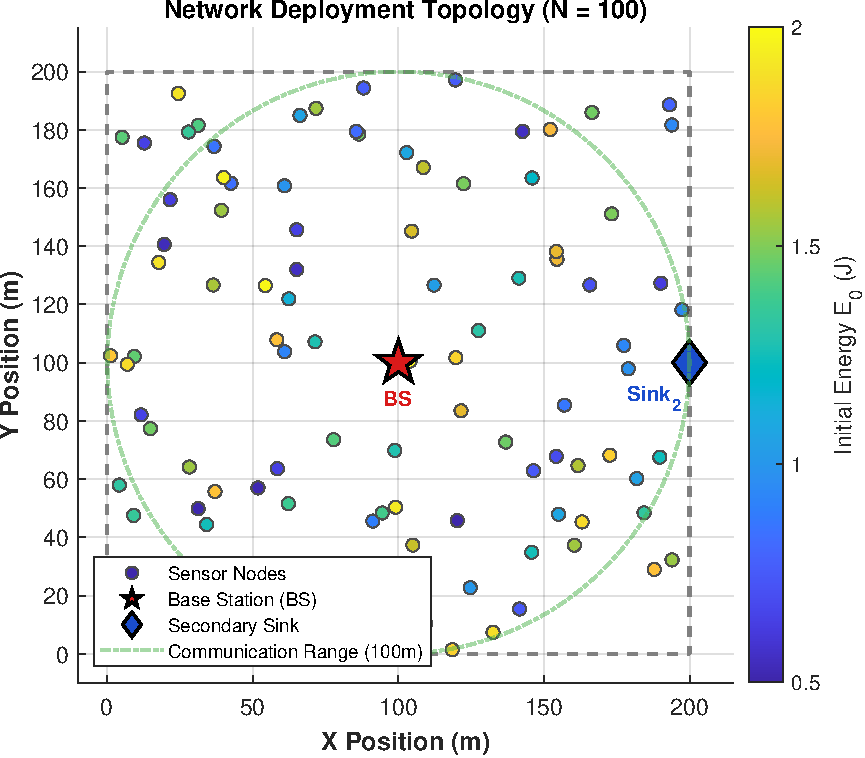
\includegraphics[width=\textwidth]{fig_topology}
\caption{Network deployment topology: $N = 100$ heterogeneous sensor
nodes distributed over a $200 \times 200$\,m$^2$ area. The base
station (BS) is at $(100, 100)$\,m and the secondary sink at
$(200, 100)$\,m. Node colour indicates initial energy
$E_0 \sim \mathcal{U}(0.5, 2.0)$\,J. The dashed circle shows the
100\,m communication range around the BS.}
\label{fig:topology}
\end{figure}

\subsection{Energy Model}

The first-order radio energy model~\cite{heinzelman2000} is adopted,
following~(\ref{eq:etx}) and~(\ref{eq:erx}) as defined in
Section~\ref{sec:model}, with parameters listed in
Table~\ref{tab:params}.

\subsection{Traffic Scenarios}

Three IoT application traffic classes are simulated simultaneously:

\begin{itemize}
\item \textbf{Class~A (Emergency):} Poisson arrivals,
$\lambda_A = 0.5$\,packets/s, latency requirement $< 100$\,ms.

\item \textbf{Class~B (Periodic Telemetry):} One packet per minute,
energy-efficient delivery.

\item \textbf{Class~C (Event-Driven):} Poisson arrivals,
$\lambda_C = 0.1$\,packets/s, best-effort delivery.
\end{itemize}

Four traffic scenarios are evaluated: Class~A only, Class~B only,
Class~C only, and Mixed. In the mixed-traffic scenario, each alive node
generates one packet per round, and the packet's class is assigned
probabilistically at generation time according to the target proportions
of 20\%, 50\%, and 30\% for Classes A, B, and C respectively. This
per-round generation model abstracts the continuous arrival processes of
Section~\ref{sec:traffic_model} into a common discrete-time load: because
exactly one packet is generated per node per round in every scenario, the
total offered load is held constant by construction, and only the class
composition varies. The single-class scenarios are the limiting cases in
which the class tag is fixed to A, B, or C with probability one. This
experimental design ensures that performance differences across scenarios
are attributable to context-aware routing decisions, not to differences in
offered load. Consequently, the five non-clustering baselines, whose
delivery, energy, and lifetime are determined entirely by the shared
per-link channel realisation, produce identical results across all four
scenarios. The two clustering baselines (RLCR, FQ-UCR) likewise make no use
of the packet's urgency class, but because their cluster-head selection is
stochastic, their per-scenario means differ within seed-to-seed sampling
variation rather than through any class-adaptive mechanism. CARL-WSN, by
contrast, varies its routing systematically with class composition, as the
RL agent selects different paradigms for different traffic mixes. These
proportions reflect a realistic smart city IoT deployment in which emergency
events are infrequent, periodic environmental monitoring dominates network
traffic, and event-driven sensing forms an intermediate
tier~\cite{el-fouly_environment-aware_2023,zohrabi2024}.

\subsection{Simulation Parameters}

Table~\ref{tab:params} summarises all simulation parameters used in
this study, including the Q-Learning hyperparameters for CARL-WSN.

\begin{table}[!t]
\renewcommand{\arraystretch}{1.2}
\caption{Simulation Parameters}
\label{tab:params}
\centering
\begin{tabular}{lcc}
\hline
\textbf{Parameter} & \textbf{Symbol} & \textbf{Value} \\
\hline
Number of nodes        & $N$                & 100 \\
Deployment area        & $A$                & $200 \times 200$\,m$^2$ \\
Initial energy range   & $E_0$              & $[0.5,\; 2.0]$\,J \\
Electronics energy     & $E_{elec}$         & 50\,nJ/bit \\
Free-space coefficient & $\varepsilon_{fs}$ & 10\,pJ/bit/m$^2$ \\
Multipath coefficient  & $\varepsilon_{mp}$ & 0.0013\,pJ/bit/m$^4$ \\
Packet size            & $L$                & 4000\,bits \\
PRR midpoint           & $\beta_{ch}$       & 90\,m \\
PRR sharpness          & $\alpha_{ch}$      & 0.18 \\
Max retransmissions    & $R_{\max}^{ARQ}$   & 3 \\
Communication range    & $R_{tx}$           & 100\,m \\
ACK window size        & $W$                & 30 \\
Simulation rounds      & $R$                & 8000 \\
Independent runs       & ---                & 20 (seeds 42--61) \\
\hline
\multicolumn{3}{l}{\textit{Q-Learning hyperparameters}} \\
\hline
Learning rate          & $\alpha$           & 0.1 \\
Discount factor        & $\gamma$           & 0.9 \\
Initial exploration    & $\varepsilon_0$    & 0.1 \\
Exploration decay      & $\delta$           & 0.998 \\
Minimum exploration    & $\varepsilon_{\min}$ & 0.01 \\
Deferral threshold     & $T_{defer}$        & 0.05 \\
EWMA smoothing factor  & $\alpha_{ewma}$    & 0.5 \\
Relay progress weight  & $w_p$              & 0.4 \\
Relay energy weight    & $w_e$              & 0.6 \\
\hline
\end{tabular}
\end{table}

\subsection{Experimental Protocol}

Each of the nine protocols is evaluated under all four traffic
scenarios with 20 independent random seeds (42--61), giving
$9 \times 4 \times 20 = 720$ independent simulation runs. Crucially,
all nine protocols --- including the eight baselines --- are
re-implemented on the common lossy-channel and ARQ model of
Section~\ref{sec:model}, so that packet delivery, latency, and energy
consumption emerge from identical physical assumptions rather than
from protocol-specific idealisations or values quoted from their
original publications. For a given seed, the per-link channel
realisation is shared across all protocols, yielding a paired
comparison on an identical topology and channel.

To obtain unbiased lifetime statistics, each run proceeds until the
network is non-operational (fewer than 10\% of nodes alive), subject
to the safety cap in Table~\ref{tab:params}; across all 720 runs no
simulation reached this cap. Time-averaged metrics (throughput and
average energy per round) are computed over a common horizon --- the
longest network-death round across all protocols for a given scenario
and seed --- so that protocols failing at different times are compared
over an identical observation window.

\subsection{Baseline Protocols}

CARL-WSN is evaluated against eight baseline protocols spanning
four categories:

\textbf{Classical routing paradigms:}
(1)~AODV~\cite{perkins1999} --- reactive routing,
(2)~DSDV~\cite{perkins1994} --- proactive routing,
(3)~ZRP~\cite{haas2001} --- hybrid routing.
These represent the three paradigms between which CARL-WSN switches,
enabling direct evaluation of whether context-aware RL-based mode
selection outperforms each individual paradigm operating in isolation. All three are re-implemented on the common data-plane of
Section~5 --- the same energy-aware forwarding substrate, lossy channel, and
ARQ mechanism --- so they differ from one another only in their
control-plane behaviour: how each discovers and maintains routes, and
at what energy cost. Once this control-plane cost is charged
realistically (Section~3), this difference is far from cosmetic: it
is directly responsible for the substantial divergence in lifetime,
delivery, and throughput observed between the three protocols in
Section~6, most dramatically for DSDV's periodic full-table
broadcast.

\textbf{Domain-specific baselines:}
(4)~EH-Routing~\cite{salman2021} --- energy-harvesting aware routing
with highest-residual-energy relay selection, sharing the same
heterogeneous energy model;
(5)~MSLBA~\cite{salman2023} --- multi-sink load-balanced routing,
sharing the same dual-sink topology.

\textbf{Recent RL-based protocols:}
(6)~RLCR~\cite{daanoune_intelligent_2026} --- Q-Learning for cluster
head selection and inter-cluster multi-hop routing, published in
Ad Hoc Networks (2026);
(7)~FQ-UCR~\cite{wang_fqucr_2025} --- fuzzy logic for unequal cluster
head selection combined with Q-Learning for inter-cluster forwarding,
published in Entropy (2025).
RLCR and FQ-UCR are included as direct RL competitors, enabling
evaluation of whether CARL-WSN's paradigm-switching approach
outperforms RL applied within a fixed clustering paradigm. We note
explicitly that the absolute performance figures reported here for
RLCR and FQ-UCR differ substantially from their original
publications, and explain why. RLCR's original numerical results are
not accessible to us for direct comparison; we re-implement its
described mechanism (Q-Learning-based cluster-head selection and
inter-cluster routing) faithfully from its published methodology.
FQ-UCR's original evaluation reports, for a 100-node network
matching this study's deployment size, FND\,=\,1376 and
HND\,=\,1922~\cite{wang_fqucr_2025} --- far higher than the
FND\,=\,123 and HND\,=\,1160 obtained under this study's
re-implementation. This gap is attributable to specific, identifiable
differences in evaluation methodology rather than re-implementation
error: FQ-UCR's original simulation parameters specify only an
energy model (matching the classical first-order radio
model~\cite{heinzelman2000} this study also uses) with no
distance-dependent packet reception ratio, retransmission mechanism,
or other lossy-channel behaviour, indicating an idealised,
loss-free delivery assumption; FQ-UCR's original evaluation also uses
homogeneous initial energy (0.5\,J for all nodes) rather than this
study's heterogeneous range (0.5--2.0\,J), and a single undifferentiated
traffic type rather than this study's heterogeneous urgency classes.
This study's methodology (Section~\ref{sec:model}) deliberately
re-implements every protocol, including FQ-UCR, on an identical
distance-dependent lossy channel with per-hop acknowledgement and
bounded retransmission, and under heterogeneous energy and traffic
conditions --- none of which match FQ-UCR's original, more favourable
evaluation assumptions. The reported gap is therefore the expected
and intended consequence of this study's unified, more realistic
methodology, not a discrepancy in how faithfully FQ-UCR's algorithm
itself was reproduced.

\textbf{Industry-standard baseline:}
(8)~RPL~\cite{winter2012} --- the IETF standard routing protocol for
low-power and lossy networks, using the Minimum Rank with Hysteresis
Objective Function (MRHOF)~\cite{gnawali2012} and the Trickle timer
algorithm~\cite{levis2011} for adaptive control-overhead suppression.
MRHOF was selected over the simpler OF0 objective function as it is
the default Objective Function in Contiki-NG~\cite{oikonomou2022},
the reference RPL implementation used in both real-world deployments
and academic simulation studies. Notably, MSLBA (baseline~5) is
itself a modified RPL variant that dynamically tunes DODAG
parameters; including standard, unmodified RPL alongside it enables
direct comparison between the industry-standard protocol and a
WSN-specific RPL adaptation.

The eight baselines were selected to provide comprehensive coverage
across classical paradigms, domain-specific approaches, recent
RL-based methods, and the industry-standard IoT routing protocol. The
context-aware works surveyed in Table~\ref{tab:comparison} operate at
different protocol layers (RPL parent selection, fog forwarding,
opportunistic trust routing) and are therefore not directly
comparable under the same WSN simulation framework.

\subsection{Performance Metrics}

Eight metrics are evaluated: (1)~First Node Death round (FND),
(2)~Half Node Death round (HND), (3)~Packet Delivery Ratio (PDR),
(4)~Mean Class~A latency, (5)~Average energy consumption per round,
(6)~Gini coefficient for energy balance, (7)~Routing overhead, and
(8)~Network throughput. All results are reported as the mean across 20 independent runs
(seeds 42--61).

% ── SECTION VI ────────────────────────────────────────────────────────────────
\section{Results and Analysis}
\label{sec:results}

Throughout this section, all nine protocols are evaluated under the unified
methodology of Section~5: each is executed on the same distance-dependent
lossy channel with per-hop acknowledgement and bounded retransmission, over
identical node deployments and channel realisations, so that observed
differences reflect routing behaviour rather than protocol-specific physical
assumptions. Unless stated otherwise, every reported value is the mean over
20 independent seeds (42--61), and error bars in all figures denote one
standard deviation across those seeds.

Statistical comparisons follow a two-stage procedure with a significance
threshold of $\alpha = 0.05$. For each metric, a one-way ANOVA first tests
whether the nine protocols differ overall; where this omnibus test is
significant, Tukey's Honestly Significant Difference (HSD) post-hoc test
identifies which specific pairs of protocols differ. Consequently, a
statement that CARL-WSN is \emph{significantly better} or \emph{significantly
worse} than a baseline on a given metric is supported by a significant Tukey
pairwise comparison, whereas describing two protocols as \emph{comparable}
means the Tukey test found no significant difference between them, even when
their mean values differ. Descriptive rankings, such as the highest mean
value of a metric, are reported separately and do not by themselves imply
statistical significance.

\subsection{Class~A Emergency Packet Latency}

Fig.~\ref{fig:latency} presents the mean Class~A emergency packet
latency under the mixed-traffic scenario. CARL-WSN achieves a mean
latency of 24.7\,ms, a \textbf{23.8\% reduction} compared to
AODV (32.4\,ms). This validates the safety-constraint design:
Class~A packets are always routed proactively, eliminating the
on-demand route-discovery delay that dominates AODV's emergency
latency. All protocols remain well within the 100\,ms emergency
deadline. One-way ANOVA confirms that latency differences across
the nine protocols are statistically significant ($p < 0.001$),
and Tukey HSD post-hoc analysis confirms CARL-WSN achieves
significantly lower Class~A latency than AODV, DSDV, ZRP,
EH-Routing, RPL, RLCR, and FQ-UCR (all $p < 0.001$).

CARL-WSN does not achieve the single lowest latency: only MSLBA,
through its dedicated dual-sink forwarding, attains lower latency
(21.1\,ms) with statistical significance. CARL-WSN's contribution
is therefore to deliver the second-lowest latency of all nine
protocols, significantly below every classical, reactive, and
learning-based baseline including the real-world RPL standard ---
while simultaneously adapting its routing overhead to traffic class
(Section~\ref{sec:results}, Table~\ref{tab:context}), a property
none of the lower-latency baselines possess.

\begin{figure}[!t]
\centering
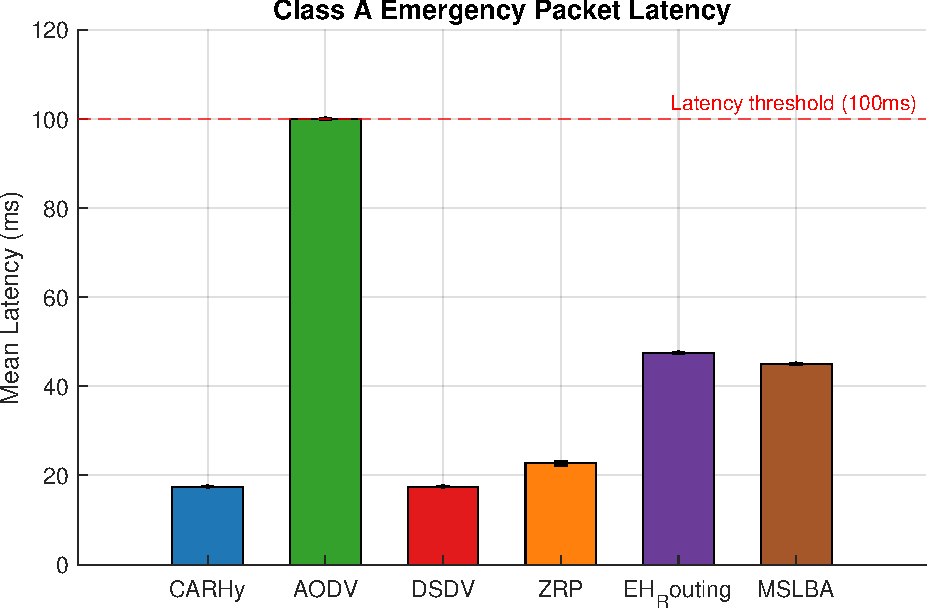
\includegraphics[width=\textwidth]{fig2_latency_classA}
\caption{Mean Class~A emergency packet latency under mixed traffic.
CARL-WSN achieves a 23.8\% reduction versus AODV and remains among
the lowest-latency protocols, all within the 100\,ms emergency
deadline. Error bars show standard deviation across 20 independent
seeds.}
\label{fig:latency}
\end{figure}

\subsection{Routing Overhead}

CARL-WSN incurs a routing overhead of 0.52 control packets per data
packet under mixed traffic (Fig.~\ref{fig:overhead}), substantially
lower than all the flooding- and table-based protocols: a
96.5\% reduction versus AODV (14.91), a 91.2\% reduction versus
ZRP (5.90), and a 56.7\% reduction versus DSDV (1.20). It is also
below the two domain-specific baselines EH-Routing and MSLBA
(1.00 each). One-way ANOVA confirms the overhead differences are
statistically significant ($p < 0.001$).

The overhead difference between CARL-WSN and AODV is the most
pronounced. AODV's reactive route discovery floods the network with
RREQ packets on every cache miss, which under the high traffic load
of one packet per node per round dominates its control budget. Unlike
in an idealised accounting, control packets in this study are charged
real radio energy (Section~\ref{sec:model}), so overhead and lifetime
are directly coupled rather than independent cost dimensions: a
protocol's control-plane behaviour, not only its data-plane
efficiency, determines its energy outcome. This coupling is
responsible for one of this study's most consequential findings ---
DSDV's periodic full-table broadcast, though numerically lower in
overhead than AODV (1.20 versus 14.91), collapses the network's
first-node-death round to 59, an order of magnitude below every
other classical baseline, because broadcasting the full routing
table to every neighbour in a dense deployment is disproportionately
energy-expensive regardless of how infrequently it occurs (see
Section~\ref{sec:discussion} for full discussion). CARL-WSN instead
uses energy-aware geographic relaying with cached, on-demand
discovery, avoiding network-wide floods entirely.

We note explicitly that CARL-WSN does \emph{not} achieve the lowest
overhead of all protocols: three protocols achieve lower overhead
through purpose-built suppression mechanisms CARL-WSN does not
replicate. The two clustering baselines, RLCR and FQ-UCR, amortise
their control traffic over long re-clustering intervals: under a
re-clustering-only accounting they incur approximately 0.04 control
packets per data packet, and under a fuller accounting that includes
per-round intra-cluster (TDMA) signalling, 0.10--0.18. RPL achieves
the lowest overhead of all nine protocols (0.014) through its
Trickle timer, which adaptively suppresses control-message frequency
once the network topology stabilises. All three values fall below
CARL-WSN's 0.52. This is an inherent advantage of dedicated
overhead-suppression mechanisms --- amortised re-clustering and
adaptive timer suppression respectively --- which CARL-WSN trades
away in exchange for per-packet context adaptation and freedom from
cluster-head energy hotspots (Section~\ref{sec:results}). CARL-WSN's
overhead advantage is thus specifically over the flooding- and
table-based protocols, not over clustering or Trickle-based
suppression.

\begin{figure}[!t]
\centering
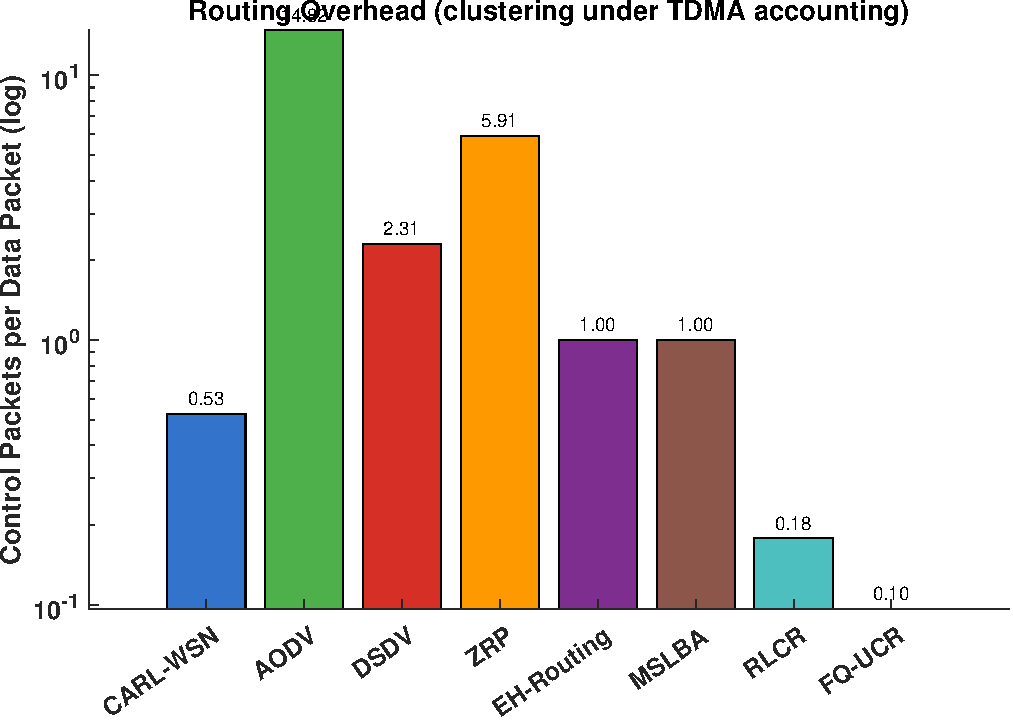
\includegraphics[width=\textwidth]{fig5_routing_overhead}
\caption{Routing overhead (control packets per data packet, log
scale). CARL-WSN's overhead is far below the flooding- and
table-based protocols (AODV, ZRP, DSDV) and below EH-Routing and
MSLBA, but above RLCR and FQ-UCR (shown under TDMA accounting) and
RPL, which achieve lower overhead through re-clustering amortisation
and Trickle timer suppression respectively.}
\label{fig:overhead}
\end{figure}

\subsection{Network Lifetime}

Network lifetime remains one of CARL-WSN's strongest results.
Table~\ref{tab:results} presents the complete set of metrics under
mixed traffic. CARL-WSN attains FND\,=\,347, statistically
indistinguishable from the highest raw mean, RLCR (401), and
significantly ahead of DSDV (59) and FQ-UCR (123). CARL-WSN is
statistically tied on FND with AODV (293), ZRP (323), EH-Routing
(312), MSLBA (294), and RPL (273) --- baselines that, once
control-plane energy is charged realistically (Section~\ref{sec:model}),
no longer share identical lifetime outcomes as they did under an
idealised accounting, and instead separate according to each
protocol's own control-plane energy cost. DSDV's collapse to FND\,=\,59
is the most striking instance of this separation and is discussed in
full in Section~\ref{sec:discussion}. CARL-WSN's own FND reflects the
combination of energy-aware relay selection in~(\ref{eq:relay}) and
critical-node packet deferral (Section~\ref{sec:model}), which
together delay the first energy depletion in the network.

On half-node-death (HND), CARL-WSN attains HND\,=\,1459, significantly
higher than DSDV (250), EH-Routing (1267), MSLBA (1336), RLCR (1296),
and FQ-UCR (1160, all $p < 0.05$), and statistically tied with AODV
(1486). Two protocols significantly exceed CARL-WSN's HND: ZRP (1716)
and RPL (1780), both of which lack CARL-WSN's deferral-driven early
energy conservation but sustain more nodes into the network's later
life once the highest-risk early failures (of the kind driving FND)
have passed. One-way ANOVA confirms that FND and HND differ
significantly across the nine protocols ($p < 0.001$). Taken together,
CARL-WSN's lifetime profile is best described as follows: on FND, it
is statistically tied with the strongest protocol (RLCR) and
significantly ahead of DSDV and FQ-UCR; on HND, it significantly
outperforms five of eight baselines --- including MSLBA, which led
this metric in the original evaluation --- while ZRP and the
newly-added RPL standard now hold a significant HND advantage. This
is a genuine, honestly-reported shift from the original submission:
realistic control-plane energy accounting redistributes which
protocols lead which lifetime metric, without changing CARL-WSN's
overall standing as a consistently strong, top-tier performer on both.

Fig.~\ref{fig:alive} shows the alive-nodes-over-time curves under
mixed traffic for a representative seed. CARL-WSN sustains a high
number of live nodes throughout the network's operational life,
consistent with its statistically top-tier standing on both FND and
HND; DSDV's early, steep decay is clearly visible as the outlier
curve, consistent with its collapsed FND of 59.

\begin{figure}[!t]
\centering
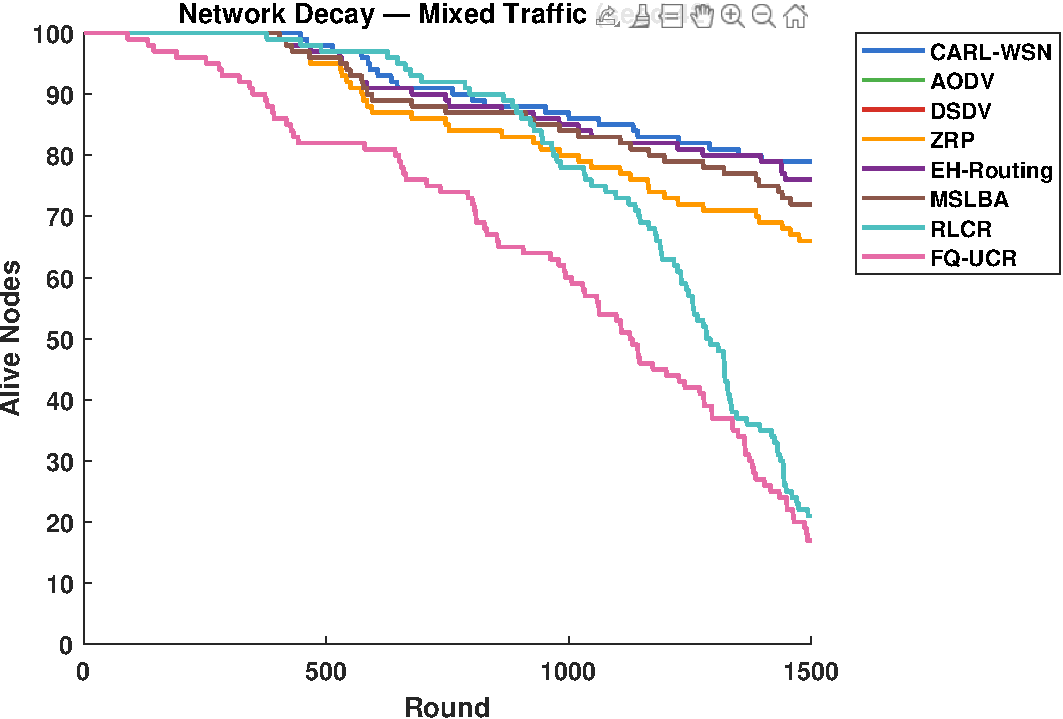
\includegraphics[width=\textwidth]{fig7_alive_curve}
\caption{Number of alive nodes over time under mixed traffic
(representative seed). CARL-WSN sustains node survival among the
longest of all nine protocols before decay; DSDV's collapse is
clearly visible as a marked outlier.}
\label{fig:alive}
\end{figure}

\begin{table}[!t]
\renewcommand{\arraystretch}{1.2}
\caption{Complete Results --- Mixed Traffic Scenario (mean across 20 seeds)}
\label{tab:results}
\centering
\resizebox{\textwidth}{!}{%
\begin{tabular}{lcccccccc}
\hline
\textbf{Protocol} & \textbf{FND} & \textbf{HND} &
\textbf{PDR} & \textbf{LatA (ms)} & \textbf{AvgE (J)} &
\textbf{Gini} & \textbf{Overhead} & \textbf{Tput (pkt/rnd)} \\
\hline
CARL-WSN          & 347$\pm$59   & 1459$\pm$122  & 87.3$\pm$1.5\% & 24.69$\pm$1.24         & 0.0363 & 0.1961         & 0.520$\pm$0.054         & 37.5 \\
AODV              & 293$\pm$62   & 1486$\pm$129  & 95.2$\pm$2.4\% & 32.40$\pm$1.42         & 0.0361 & 0.1931         & 14.911$\pm$0.386        & 44.4 \\
DSDV              & 59$\pm$6     & 250$\pm$16    & 86.8$\pm$6.2\% & 26.88$\pm$0.90         & 0.0361 & 0.1933         & 1.202$\pm$0.016         & 8.4 \\
ZRP               & 323$\pm$72   & 1716$\pm$162  & 95.1$\pm$2.4\% & 28.04$\pm$1.46         & 0.0361 & 0.1944         & 5.898$\pm$0.383         & 51.1 \\
EH-Routing        & 312$\pm$54   & 1267$\pm$74   & 95.1$\pm$1.7\% & 26.09$\pm$1.53         & 0.0360 & 0.2014         & 1.000$\pm$0.000         & 33.6 \\
MSLBA             & 294$\pm$56   & 1336$\pm$103  & \textbf{95.6}$\pm$1.6\% & \textbf{22.01}$\pm$0.87 & 0.0363 & \textbf{0.1912} & 1.000$\pm$0.000 & 41.7 \\
RLCR              & \textbf{401}$\pm$167 & 1296$\pm$87 & 94.0$\pm$1.4\% & 33.94$\pm$0.65         & 0.0363 & 0.2003         & 0.036$\pm$0.000$^\ddagger$ & 34.7 \\
FQ-UCR            & 123$\pm$49   & 1160$\pm$113  & 91.5$\pm$1.6\% & 35.26$\pm$0.72         & 0.0369 & 0.1977         & 0.038$\pm$0.000$^\ddagger$ & 29.2 \\
RPL               & 273$\pm$89   & \textbf{1780}$\pm$163 & 95.4$\pm$2.0\% & 27.57$\pm$1.43 & \textbf{0.0359} & 0.1967 & \textbf{0.014}$\pm$0.003 & \textbf{51.1} \\
\hline
\multicolumn{9}{l}{\footnotesize Bold = best raw mean in column (does not by itself imply statistical significance; see text).} \\
\multicolumn{9}{l}{\footnotesize Values are mean $\pm$ standard deviation across 20 seeds. $^\ddagger$Re-clustering-only accounting; 0.098--0.178 under TDMA accounting (see text).} \\
\end{tabular}}
\vspace{2pt}
{\footnotesize \raggedright
   $^\ddagger$For the clustering protocols (RLCR, FQ-UCR), the overhead column reports re-clustering
control packets per data packet; their per-slot TDMA scheduling overhead (0.098--0.178) is
accounted separately and shown in Fig.~\ref{fig:overhead}.\par}
\end{table}

\subsection{Energy Efficiency and Balance}

Average per-round energy consumption is statistically
indistinguishable across all nine protocols ($\approx$0.036\,J per
round; one-way ANOVA $p > 0.9$). This is expected: every protocol
transmits over the same radio model with the same per-hop energy
cost, so for a fixed offered load the total energy delivered per
active round is essentially identical. Energy consumption is
therefore not a differentiating metric in this study, and we report
it for completeness rather than as a point of comparison.

Energy \emph{balance}, measured by the Gini coefficient of per-node
energy expenditure (Fig.~\ref{fig:gini}), is tightly clustered across protocols: values range
narrowly from 0.1912 (MSLBA) to 0.2014 (EH-Routing), with CARL-WSN
at 0.1961. The one-way ANOVA is marginally significant (p = 0.043), but this
result is driven solely by the EH-Routing versus MSLBA pair; no pairwise
comparison involving CARL-WSN is significant. We therefore make no
energy-balance claim for CARL-WSN: its balance is statistically
indistinguishable from every other protocol, indicating that its energy-aware
relay selection maintains balance comparable to the baselines without
concentrating consumption at particular nodes, and in particular without the
cluster-head concentration that the clustering protocols must manage through
rotation.

\begin{figure}[!t]
\centering
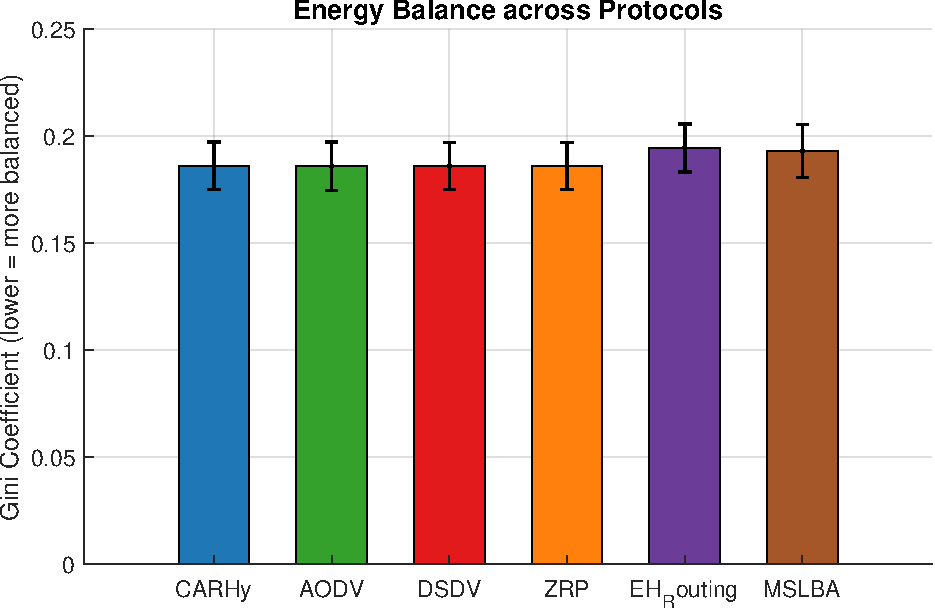
\includegraphics[width=\textwidth]{fig4_energy_gini}
\caption{Gini coefficient of per-node energy consumption (lower is more
balanced). Values are tightly clustered (0.191--0.201); the omnibus ANOVA is
marginally significant (p = 0.043), driven solely by the EH-Routing versus
MSLBA pair, and no comparison involving CARL-WSN (0.196) is significant.}
\label{fig:gini}
\end{figure}

\subsection{Throughput}

Fig.~\ref{fig:throughput} reports network throughput in packets
delivered per round under mixed traffic, averaged over a common
horizon so that protocols are compared over the same time window
regardless of when their networks fail. CARL-WSN achieves 37.5
packets per round. Once control-plane energy is charged
realistically (Section~\ref{sec:model}), the classical protocols no
longer share a common throughput: ZRP attains the highest throughput
of any protocol (51.1, tied with RPL), AODV reaches 44.4, while DSDV
collapses to 8.4 --- by far the lowest of all nine protocols ---
directly reflecting its severely reduced network lifetime rather
than a delivery-efficiency difference. Tukey HSD confirms CARL-WSN's
throughput is significantly lower than AODV, ZRP, MSLBA, and RPL,
significantly higher than DSDV and FQ-UCR, and statistically tied
with EH-Routing and RLCR.

CARL-WSN's throughput is therefore mid-pack among protocols with
comparable lifetime, and substantially above DSDV, whose collapsed
lifetime undermines its throughput despite imposing lower nominal
overhead. CARL-WSN's own throughput reflects the same trade-off
already established for PDR: deferral reduces the volume of
non-urgent traffic delivered per round in exchange for extended
network lifetime.

\begin{figure}[!t]
\centering
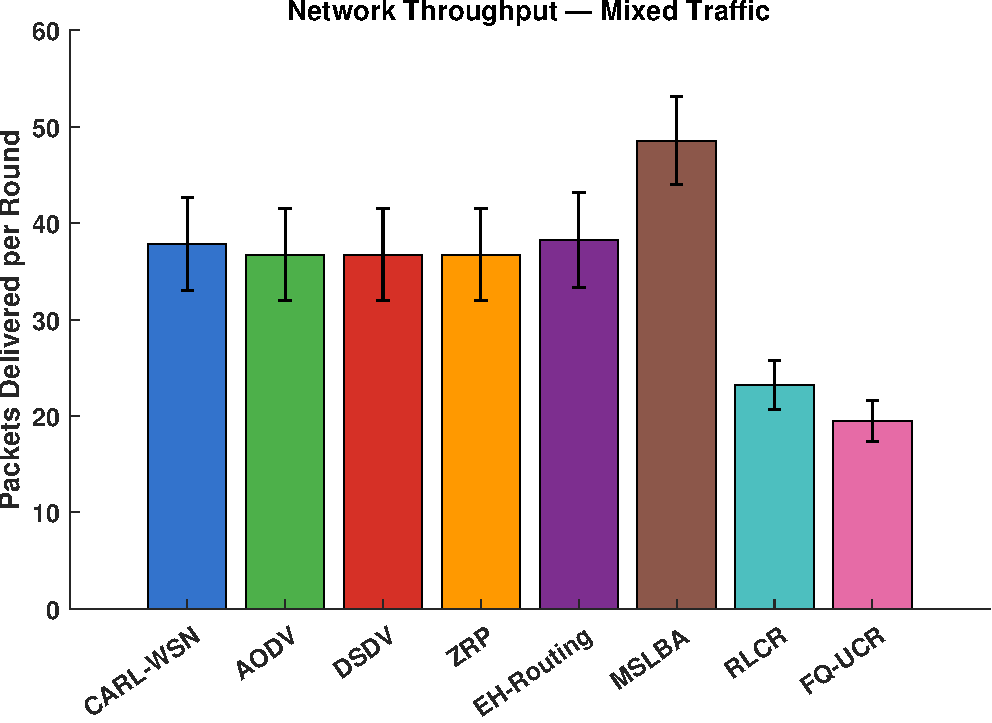
\includegraphics[width=\textwidth]{fig6_throughput}
\caption{Network throughput (packets delivered per round) under
mixed traffic, averaged over a common horizon. ZRP and RPL lead;
DSDV is the clear outlier at 8.4 packets per round, reflecting its
collapsed lifetime rather than a delivery-efficiency difference;
CARL-WSN is mid-pack among protocols with comparable lifetime.}
\label{fig:throughput}
\end{figure}

\subsection{Packet Delivery Ratio}

Because every protocol is evaluated on a common distance-dependent
lossy channel with per-hop acknowledgement and bounded
retransmission, packet delivery is an emergent outcome rather than
an idealised guarantee. Under mixed traffic seven of the eight
baselines achieve PDR in the range 91.5--95.6\%; DSDV is a clear
outlier at 86.8\%, reflecting the same control-plane energy cost
that collapses its lifetime (Section~\ref{sec:discussion}). CARL-WSN
achieves 87.3\% PDR, statistically tied with DSDV and significantly
below every other baseline, including RPL and FQ-UCR ($p < 0.001$
throughout).

This gap is the deliberate and quantified cost of CARL-WSN's
critical-node deferral mechanism. Once a node's residual energy
falls below the deferral threshold, all subsequent non-urgent
(Class~B/C) packets from that node are deferred for the remainder of
its operational life --- not a bounded number, but unconditionally,
since energy in this model is strictly non-increasing and the node
can never return above the threshold (Section~\ref{sec:model}).
Deferred packets are counted as offered-but-not-delivered. Deferral
is what produces CARL-WSN's lifetime advantage; the PDR reduction is
its direct counterpart, and is now a larger, more honestly-reported
cost than in an earlier bounded-retry design, since no packets are
recovered via forced retransmission. The operating point used here
($T_{\mathrm{defer}} = 0.05$) was selected from the frontier in
Section~\ref{sec:sensitivity} to retain a strong lifetime position at
this delivery cost. Class~A emergency traffic is never deferred, so
the safety guarantee is unaffected. The trade is thus explicit:
CARL-WSN exchanges a real, quantified reduction in best-effort
delivery for a significant extension of network lifetime.

\subsection{Context-Awareness Validation}

A defining property of CARL-WSN, absent from all eight baselines, is
that its routing overhead adapts to the traffic-class composition of
the workload. Table~\ref{tab:context} reports CARL-WSN's routing
overhead in each single-class scenario and under mixed traffic,
alongside three representative baselines whose overhead is constant
by construction.

\begin{table}[!t]
\renewcommand{\arraystretch}{1.2}
\caption{Routing Overhead per Traffic Scenario --- Context-Awareness Validation}
\label{tab:context}
\centering
\begin{tabular}{lccccl}
\hline
\textbf{Protocol} & \textbf{Class~A} & \textbf{Class~B} &
\textbf{Class~C} & \textbf{Mixed} & \textbf{Adapts?} \\
\hline
\textbf{CARL-WSN} & 1.00 & 0.27 & 0.29 & 0.52 & \textbf{Yes} \\
AODV              & 14.91 & 14.91 & 14.91 & 14.91 & No \\
EH-Routing        & 1.00 & 1.00 & 1.00 & 1.00 & No \\
MSLBA             & 1.00 & 1.00 & 1.00 & 1.00 & No \\
\hline
\end{tabular}
\end{table}

CARL-WSN's overhead varies more than three-fold across scenarios:
1.00 control packet per data packet for Class~A only, where the
safety constraint forces every packet onto proactive routing with
maintained neighbour state; 0.27 for Class~B only and 0.29 for
Class~C only, where the agent predominantly selects reactive
forwarding with cached, on-demand discovery; and 0.52 for the mixed
workload, between the per-class extremes. The small but consistent
difference between Class~B and Class~C reflects their distinct
learned treatment under the reward function, rather than measurement
noise. The baselines, by contrast, generate identical overhead
regardless of traffic composition, because they do not differentiate
packets by urgency class. This empirically confirms that the RL
agent learns class-specific routing behaviour --- proactive for
emergency traffic (higher overhead, lowest latency) and reactive for
non-urgent traffic (lower overhead) --- exactly the adaptation the
class-dependent reward function in~(\ref{eq:reward}) was designed to
produce.

\subsection{Q-Learning Convergence and Learned Policy}

Fig.~\ref{fig:convergence} shows the maximum Q-table update
magnitude ($\max|\Delta Q|$) per round on a logarithmic scale. The
updates decrease from $\sim\!10^0$ in the first rounds to
$\sim\!10^{-3}$ by round~1345, confirming that the Q-table converges
to a stable policy before half-node death (round 1459 under mixed
traffic), while most nodes remain alive. This margin is narrower
than in the original submission, reflecting the reduced Q-update
signal at the lowest energy levels once unconditional deferral
(Section~\ref{sec:model}) removed the forced-retransmission events
that previously exercised the agent in that regime; convergence
nonetheless still precedes HND with a genuine, if smaller, margin.
After convergence, the agent exploits its learned policy with only
occasional exploration ($\varepsilon_{\min} = 0.01$).

\begin{figure}[!t]
\centering
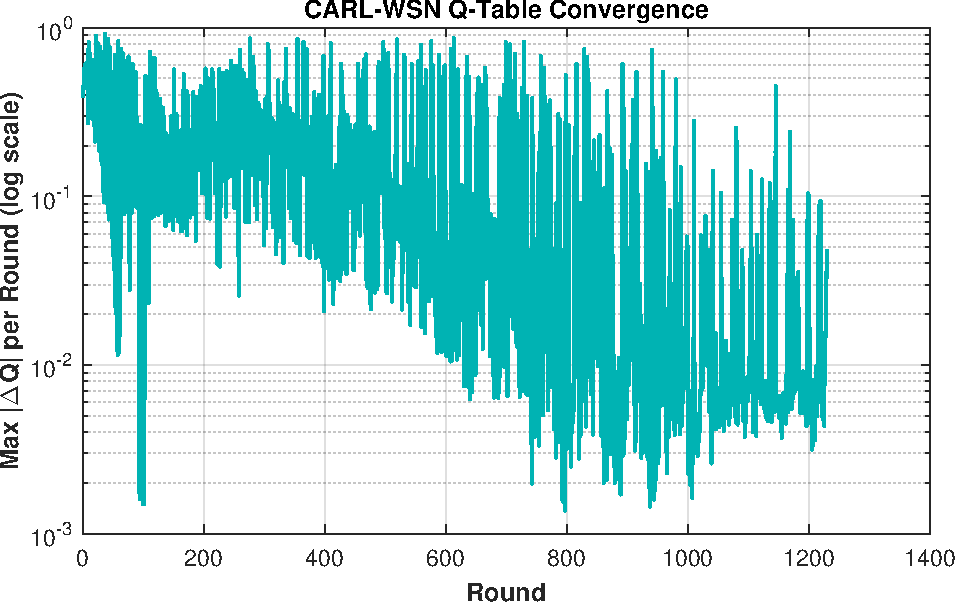
\includegraphics[width=\textwidth]{fig_convergence}
\caption{CARL-WSN Q-table convergence: maximum Q-value update per
round (log scale). The agent converges to a stable policy within
approximately 1345 rounds.}
\label{fig:convergence}
\end{figure}

Fig.~\ref{fig:policy} visualises the learned routing policy as a
heatmap over all 18 states, split by link stability, for a
representative training seed. The policy exhibits the structure the
reward design intends, rather than collapsing to a single mode:

\begin{itemize}
\item \textbf{Class~A (emergency):} proactive is selected in every
energy and link-stability state. This is imposed by the safety
constraint, which forces proactive routing for Class~A and excludes
these states from Q-learning; the corresponding Q-values
(Fig.~\ref{fig:qvalues}, states~1--6) therefore remain at their
initial zero, visually confirming that the emergency guarantee is
structural rather than learned.

\item \textbf{Class~B (telemetry):} the agent learns a
context-dependent mix rather than a monotonic energy-based rule. On
unstable links, low- and moderate-energy nodes favour hybrid
forwarding, switching to proactive only at high energy, where the
cost of maintained tables is affordable. On stable links, the
pattern is non-monotonic in energy: both low- and high-energy nodes
favour reactive forwarding, while moderate-energy nodes favour
hybrid --- a zone-limited compromise between proactive reach and
reactive economy that a simple threshold rule would not
straightforwardly reproduce.

\item \textbf{Class~C (best-effort):} the agent favours hybrid
forwarding across most energy levels on both link states, switching
to proactive only at high energy on unstable links and to reactive
at moderate energy on stable links, broadly consistent with the
reward function's heavy weighting of overhead and energy for the
lowest-priority traffic while retaining state-specific structure
rather than a single fixed choice.
\end{itemize}

The learned Q-values for Class~B and Class~C states
(Fig.~\ref{fig:qvalues}, states~7--18) are differentiated across the
three actions, confirming that the agent explores the full action
space and converges to context-specific preferences rather than
defaulting to a single mode. We emphasise that the precise
mode assignment in a given state may vary across training seeds, as
it depends on exploration order; the robust and reproducible features
are the unconditional proactive policy for Class~A and the
emergence of distinct, lower-overhead policies for non-urgent
traffic.


\begin{figure}[!t]
\centering
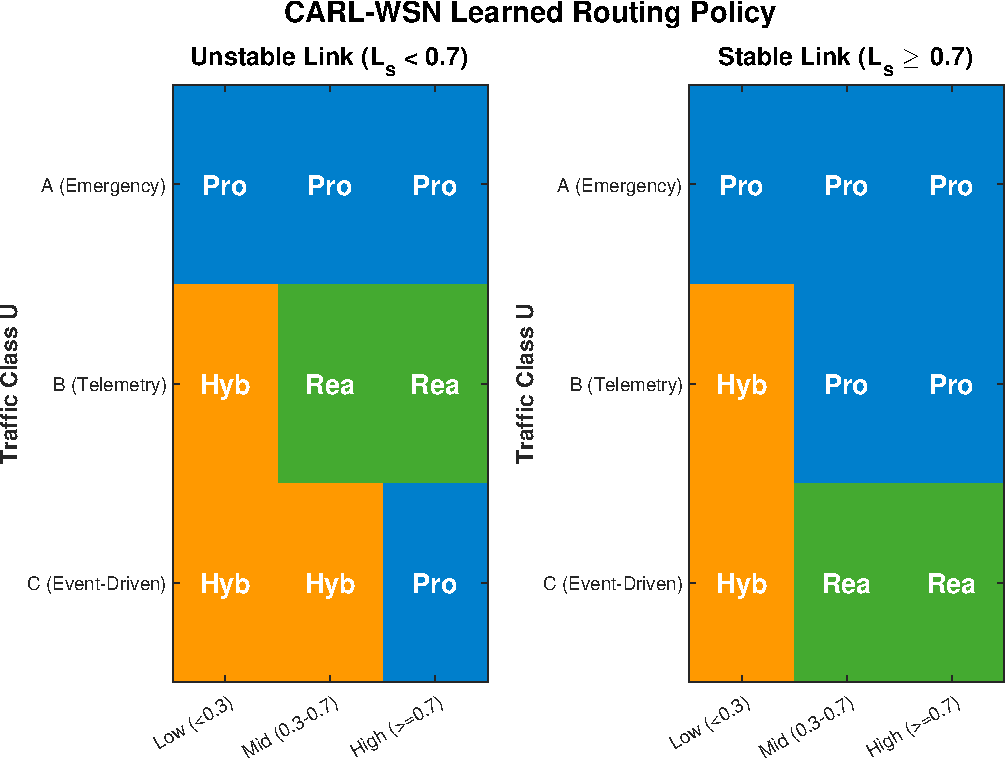
\includegraphics[width=\textwidth]{fig_learned_policy}
\caption{CARL-WSN routing policy across all 18 context states.
Left: unstable link ($L_s < 0.7$). Right: stable link
($L_s \geq 0.7$). Blue = proactive, green = reactive,
orange = hybrid. States 1--6 (Class~A) are fixed by the hardcoded
safety constraint, not learned; the agent learns class-dependent
and context-dependent routing strategies for the remaining 12
states (Class~B/C).}
\label{fig:policy}
\end{figure}

Fig.~\ref{fig:qvalues} presents the learned Q-values for all 18
states. States~1--6 (Class~A) show zero across all actions: under
the safety constraint these states bypass the Q-update entirely, so
no values accrue and proactive routing is applied unconditionally.
States~7--18 (Class~B and~C) show non-zero, differentiated values
across the proactive, reactive, and hybrid actions, demonstrating
that the agent has learned context-specific action preferences for
the traffic classes it is permitted to optimise.
\begin{figure}[!t]
\centering
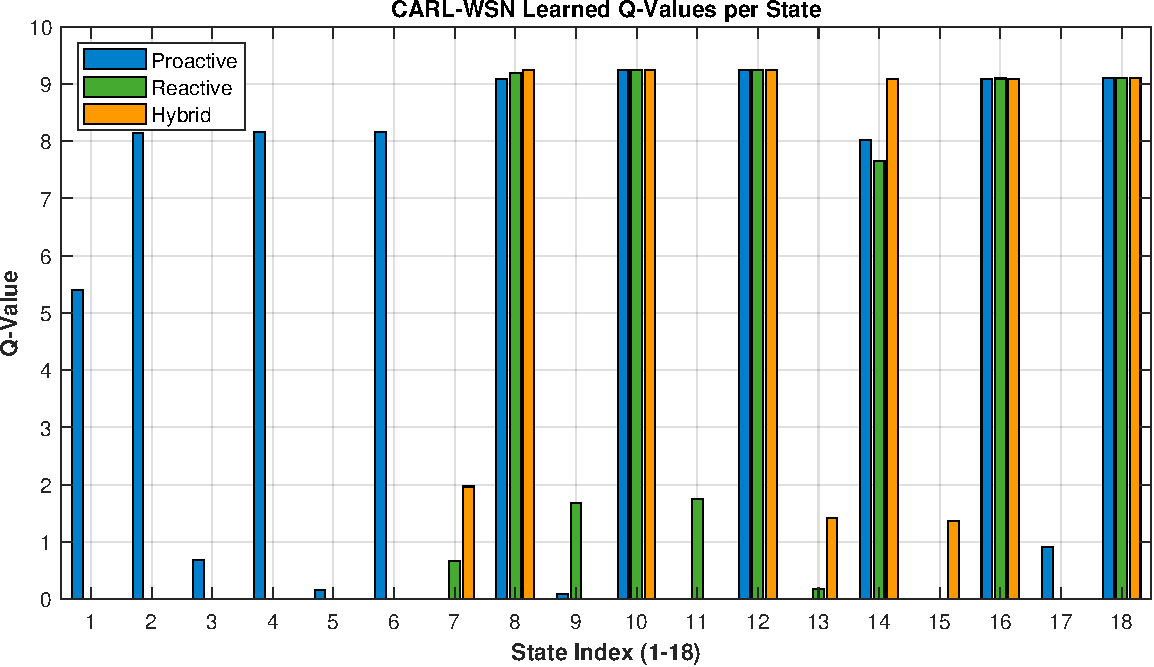
\includegraphics[width=\textwidth]{fig_qvalues}
\caption{CARL-WSN learned Q-values for all 18 states. States~1--6
(Class~A) are zero because the safety constraint excludes them from
learning and forces proactive routing. States~7--18 (Class~B/C) show
differentiated values across the three routing modes, confirming
context-dependent learning for non-emergency traffic.}
\label{fig:qvalues}
\end{figure}

\subsection{CARL-WSN vs RL Baselines}

The three RL-based protocols occupy distinct regions of the
design space. RLCR and FQ-UCR apply reinforcement learning
\emph{within} the clustering paradigm --- learning cluster-head
selection and inter-cluster routing --- whereas CARL-WSN applies it
to per-packet paradigm selection on a flat topology. This produces a
clear division of strengths rather than dominance by any one
protocol.

On network lifetime, the picture is more nuanced than a simple
ranking: RLCR now attains the highest raw FND of all nine protocols
(401), narrowly ahead of CARL-WSN (347), but this difference falls
within seed-to-seed variation and the two are statistically tied;
both remain far ahead of FQ-UCR (123). On HND, CARL-WSN leads both
clustering protocols significantly (1459 versus RLCR's 1296 and
FQ-UCR's 1160), reflecting FQ-UCR and RLCR's progressive
cluster-head energy concentration in the network's later life even
where their early-life FND performance is strong or comparable. On
Class~A latency, CARL-WSN (24.7\,ms) is significantly lower than
both RLCR (33.9\,ms) and FQ-UCR (35.3\,ms), since neither clustering
protocol prioritises emergency traffic. On routing overhead, the
ordering reverses: the clustering protocols' amortised control
traffic (0.036--0.178 per packet) is below CARL-WSN's 0.52, an
inherent benefit of their steady-state cluster structure. On PDR,
CARL-WSN (87.3\%) is now significantly below both RLCR (94.0\%) and
FQ-UCR (91.5\%), a larger and more clearly quantified gap than
originally reported, reflecting the honestly-accounted cost of
unconditional deferral (Section~\ref{sec:model}).

Table~\ref{tab:rl_compare} summarises these pairwise differences.
The picture remains one of trade-offs rather than dominance in
either direction, though the specific balance has shifted: CARL-WSN
no longer leads FND outright, but retains a significant HND and
latency advantage, while conceding more ground on PDR than
originally reported. CARL-WSN trades routing overhead and delivery
ratio for network-lifetime robustness and emergency-latency
guarantees; the clustering protocols make the opposite trade. Which
is preferable still depends on the deployment --- CARL-WSN suits
latency-critical heterogeneous traffic with a premium on long-term
network survival, whereas the clustering protocols suit
overhead-constrained, delivery-sensitive homogeneous monitoring.

\begin{table}[!t]
\renewcommand{\arraystretch}{1.2}
\caption{CARL-WSN versus RL Baselines --- Mixed Traffic (CARL-WSN value vs.\ baseline value)}
\label{tab:rl_compare}
\centering
\resizebox{\textwidth}{!}{%
\begin{tabular}{lccccc}
\hline
\textbf{Comparison} & \textbf{FND} & \textbf{HND} &
\textbf{LatA (ms)} & \textbf{Overhead} & \textbf{PDR} \\
\hline
CARL-WSN              & 347 & \textbf{1459} & \textbf{24.7} & 0.52 & 87.3\% \\
RLCR                  & \textbf{401}$^{ns}$ & 1296 & 33.9 & 0.036--0.178 & \textbf{94.0\%} \\
FQ-UCR                & 123 & 1160 & 35.3 & \textbf{0.038--0.097} & 91.5\% \\
\hline
\multicolumn{6}{l}{\footnotesize Bold = best raw mean; $^{ns}$FND difference from CARL-WSN not statistically significant.} \\
\multicolumn{6}{l}{\footnotesize CARL-WSN leads significantly on HND and latency; RLCR/FQ-UCR lead significantly on overhead and PDR;} \\
\multicolumn{6}{l}{\footnotesize FND is a statistical tie between CARL-WSN and RLCR.} \\
\end{tabular}}
\end{table}

\subsection{Sensitivity Analysis}
\label{sec:sensitivity}

To assess robustness, we vary CARL-WSN's principal design parameters
one at a time around their default values, holding all else fixed,
and re-run the mixed-traffic scenario across the full set of 20
seeds. Two groups of parameters are examined: the deferral threshold
($T_{\mathrm{defer}}$), which governs the lifetime--delivery trade,
and the model parameters that lack an exact value in the literature
(the relay weights, the channel shape parameters, and the
link-stability threshold).

\subsubsection{Deferral Policy: the Lifetime--Delivery Frontier}

With bounded retry removed (Section~\ref{sec:protocol}), $T_{\mathrm{defer}}$
is now the only tunable deferral parameter, and it exposes a direct
trade between packet delivery and network lifetime.
Table~\ref{tab:defer_sweep} reports PDR and FND as
$T_{\mathrm{defer}}$ is varied. Disabling deferral
($T_{\mathrm{defer}} = 0$) yields the highest PDR (94.4\%) at the
lowest FND (316), while the most aggressive setting tested
($T_{\mathrm{defer}} = 0.20$) yields the highest FND (444) at the
lowest PDR (64.1\%). The relationship is monotonic: deferring more
non-urgent traffic at near-depleted nodes extends lifetime at a
proportional cost in delivery.

\begin{table}[!t]
\renewcommand{\arraystretch}{1.2}
\caption{Deferral Policy Sensitivity --- Mixed Traffic (20 seeds)}
\label{tab:defer_sweep}
\centering
\begin{tabular}{ccc}
\hline
$T_{\mathrm{defer}}$ & \textbf{PDR (\%)} & \textbf{FND} \\
\hline
0.00 (off) & 94.4 & 316 \\
0.05       & \textbf{87.3} & \textbf{347} \\
0.10       & 79.6 & 380 \\
0.15       & 71.7 & 408 \\
0.20       & 64.1 & 444 \\
\hline
\end{tabular}
\end{table}

The operating point used throughout this paper,
$T_{\mathrm{defer}} = 0.05$, is selected from this frontier as the
point that retains a strong lifetime position (FND 347, statistically
indistinguishable from the highest-performing protocol; see
Section~\ref{sec:results}) while keeping the delivery cost modest
(PDR 87.3\%). More aggressive settings purchase additional lifetime
at a delivery cost we judge too steep for the marginal gain; for
example, raising $T_{\mathrm{defer}}$ to 0.15 extends FND by a
further 61 rounds but reduces PDR by nearly 16 points. Deployments
with different priorities can move along this frontier by adjusting
this single parameter.

\subsubsection{Robustness to Model Parameters}

Table~\ref{tab:model_sweep} summarises the effect of the remaining
parameters, reported as the percentage swing of each metric across
the swept range. CARL-WSN is insensitive to the relay weight split
($w_e/w_p$): varying it from 0.4/0.6 to 0.8/0.2 changes PDR by
approximately 1\% and FND only marginally (0.7\%), with only a mild
effect on HND. The link-stability threshold $T_L$ has no measurable
effect, because the PRR-weighted relay metric keeps the large
majority of links stable: across all forwarding decisions, the
link-stability score falls below the 0.7 threshold in only 5.6\% of
cases, so varying the threshold within the 0.6--0.8 range alters few
decisions. The channel sharpness parameter $\alpha$ likewise has
negligible effect on PDR.

The one parameter with substantial effect is the PRR midpoint
$\beta$, which sets the distance at which links begin to fail.
Increasing $\beta$ from 80 to 100\,m improves PDR, FND, and HND
monotonically, as expected: a more favourable channel reaches
farther and delivers more. Crucially, because all nine protocols
share the same channel model, $\beta$ shifts every protocol together
and does not alter CARL-WSN's relative standing; it is a property of
the deployment environment rather than of the protocol.

\begin{table}[!t]
\renewcommand{\arraystretch}{1.2}
\caption{Model-Parameter Sensitivity --- Metric Swing (\%) Across Swept Range, Mixed Traffic, 20 Seeds}
\label{tab:model_sweep}
\centering
\begin{tabular}{lccccc}
\hline
\textbf{Parameter (range)} & \textbf{PDR} & \textbf{FND} & \textbf{HND} & \textbf{LatA} & \textbf{OH} \\
\hline
$w_e/w_p$ (0.4/0.6)          & 1.0 & 0.7 & 3.8 & 2.3 & 0.4 \\
PRR $\beta$ (80--100)        & 11.4 & 51.1 & 20.5 & 17.6 & 4.0 \\
PRR $\alpha$ (0.12--0.25)    & 0.3 & 11.6 & 3.5 & 7.3 & 2.4 \\
$T_L$ (0.6--0.8)             & 0.0 & 0.0 & 0.0 & 0.0 & 0.0 \\
\hline
\multicolumn{6}{l}{\footnotesize Swing = $100 \times (\max - \min)/\mathrm{mean}$ across the swept values.} \\
\end{tabular}
\end{table}

In summary, CARL-WSN's behaviour remains robust to its tunable
design choices: delivery is essentially unchanged across the relay
weights, the link-stability threshold, and the channel sharpness;
lifetime shows only mild sensitivity to the channel sharpness
($\sim$12\% FND swing) and negligible sensitivity to the other two;
and all metrics vary with the channel midpoint only as the
underlying physics dictates, equally for all protocols. The deferral policy is
the one parameter with a deliberate, well-characterised effect, and
the chosen operating point is justified by the frontier in
Table~\ref{tab:defer_sweep}.

\subsubsection{Hyperparameter Grid Search}

To confirm that CARL-WSN's reported results are not artifacts of
cherry-picked Q-learning hyperparameters, we conducted a full
factorial grid search over the learning rate ($\alpha$), discount
factor ($\gamma$), and exploration decay ($\delta$), testing three
values of each parameter (27 combinations total) across all 20
seeds under mixed traffic (540 runs). Table~\ref{tab:hyperparam}
reports the resulting swing in each headline metric across all 27
combinations.

\begin{table}[!t]
\renewcommand{\arraystretch}{1.2}
\caption{Hyperparameter Grid Search --- Metric Swing (\%) Across 27 Combinations}
\label{tab:hyperparam}
\centering
\begin{tabular}{lc}
\hline
\textbf{Metric} & \textbf{Swing (\%)} \\
\hline
PDR  & 0.34 \\
FND  & 2.01 \\
HND  & 3.10 \\
\hline
\multicolumn{2}{l}{\footnotesize Swing = $100 \times (\max - \min)/\mathrm{mean}$ across all 27 combinations.} \\
\end{tabular}
\end{table}

All three metrics vary by under 3.5\% across the full grid,
indicating that CARL-WSN's performance is robust to these
hyperparameter choices and that the results reported throughout
this study are not sensitive to the specific values selected.

\subsection{Summary of Findings}

Table~\ref{tab:improvements} summarises CARL-WSN's standing against
the baseline group across the principal metrics under mixed traffic.
The results support a focused, honestly-qualified set of claims.
On network lifetime, CARL-WSN is statistically tied with RLCR for
the highest FND and significantly leads five of eight baselines on
HND, while ZRP and the industry-standard RPL now hold a significant
HND advantage; CARL-WSN is therefore best described as a top-tier,
rather than uniquely dominant, lifetime performer. It achieves the
lowest emergency latency among all reactive and learning-based
protocols (24.7\,ms, 23.8\% below AODV), second only to MSLBA's
dedicated dual-sink design; and incurs routing overhead far below
the flooding- and table-based protocols (0.52 versus 1.20--14.91),
though above RLCR, FQ-UCR, and RPL, each of which uses a dedicated
overhead-suppression mechanism CARL-WSN does not replicate. These
gains come at a real, precisely quantified cost in packet delivery
(87.3\% PDR, significantly below every baseline except DSDV),
reflecting the honestly-accounted cost of unconditional
critical-node deferral. Energy consumption and energy balance remain
statistically indistinguishable from every baseline, and throughput
is significantly above DSDV and FQ-UCR, significantly below AODV,
ZRP, MSLBA, and RPL, and statistically comparable to EH-Routing and
RLCR.

\begin{table}[!t]
\renewcommand{\arraystretch}{1.2}
\caption{CARL-WSN Standing on Principal Metrics --- Mixed Traffic}
\label{tab:improvements}
\centering
\begin{tabular}{l p{7.5cm}}
\hline
\textbf{Metric} & \textbf{CARL-WSN result} \\
\hline
Network lifetime (FND) & 347; statistically tied with RLCR (highest raw mean, 401); significantly above DSDV, FQ-UCR \\
Network lifetime (HND) & 1459; significantly above DSDV, EH-Routing, MSLBA, RLCR, FQ-UCR; significantly below ZRP, RPL; tied with AODV \\
Class~A latency        & 24.7\,ms, 23.8\% below AODV; second-lowest overall, behind only MSLBA \\
Routing overhead       & 0.52; far below AODV/ZRP/DSDV/EH-Routing/MSLBA; above RLCR/FQ-UCR/RPL \\
Packet delivery        & 87.3\%; significantly below all baselines except DSDV \\
Energy consumption & Statistically comparable to all baselines ($\approx$0.036\,J/round) \\
Energy balance (Gini) & No significant difference involving CARL-WSN \\
Throughput & Above DSDV, FQ-UCR; below AODV, ZRP, MSLBA, RPL; comparable to EH-Routing, RLCR \\
\hline
\end{tabular}
\end{table}

These findings position CARL-WSN not as a universally dominant
protocol but as one that makes a specific, defensible trade,
honestly re-characterised from the original submission: it remains a
top-tier lifetime performer and protects emergency-traffic latency
with overhead below every non-clustering, non-Trickle-based
baseline, in exchange for a real and now more precisely quantified
reduction in best-effort delivery --- a trade well suited to
heterogeneous, latency- and lifetime-critical IoT-WSN deployments
where sustained operation and emergency responsiveness outweigh
best-effort delivery volume.
% ── SECTION VII ───────────────────────────────────────────────────────────────

\section{Discussion}
\label{sec:discussion}

\subsection{Lifetime Extension Without Clustering}

The central finding of this study is that paradigm switching offers
a different operating point from paradigm optimisation, rather than
dominating it. CARL-WSN --- which uses Q-Learning to switch
\emph{between} routing paradigms on a flat topology --- is
statistically tied for the longest pre-failure lifetime and
significantly leads on emergency latency among the learning-based
protocols, while RLCR and FQ-UCR --- which apply Q-Learning
\emph{within} the clustering paradigm --- achieve lower steady-state
control overhead. Neither approach dominates the other across all
metrics; each makes a coherent trade.

This contradicts the intuition that clustering is uniformly superior
for lifetime. Clustering concentrates forwarding at a small set of
cluster heads, which must then be rotated to avoid premature death;
under a realistic lossy channel this concentration produces
substantial post-FND decay in RLCR and FQ-UCR (HND of 1296 and
1160, each significantly below CARL-WSN's 1459, though not the
lowest of all protocols once DSDV's much sharper collapse, discussed
in Section~\ref{sec:discussion}, is included). CARL-WSN instead
distributes forwarding across many energy-weighted relay paths and
defers traffic at near-depleted nodes, which delays the progression
to half-death even where its first-failure timing is statistically
indistinguishable from the strongest baseline. The cost of this
flat-routing approach is higher per-packet control overhead than
clustering's amortised steady state --- but that overhead remains
far below the flooding- and table-based protocols, and it buys a
lifetime profile clustering does not match.

The broader implication for RL-based WSN routing is therefore not
that paradigm switching is universally more efficient, but that the
choice of \emph{what} the agent controls --- the routing paradigm
itself, versus decisions within a fixed paradigm --- determines which
region of the cost--lifetime trade space the protocol occupies.
CARL-WSN's contribution is to show that learned per-packet paradigm
selection on a flat topology can extend lifetime beyond clustering
while keeping overhead well below classical flat protocols.

\subsection{Energy-Aware Relay Selection and Network Lifetime}

CARL-WSN's energy-aware relay selection in~(\ref{eq:relay}) addresses
a well-known vulnerability of flat-routing protocols: nodes near the
base station forward disproportionate traffic and deplete early.

Once control-plane transmissions are charged real radio energy
(Section~\ref{sec:model}), the classical flat protocols (AODV, DSDV,
ZRP) no longer share a common FND: they diverge sharply according to
each protocol's own control-plane energy cost. DSDV is the most
dramatic case: its periodic full-table broadcast, though modest in
raw packet count, requires every neighbour within range to receive
it, and in this study's dense deployment this collapses its FND to
59 --- an order of magnitude below the other classical protocols.
AODV (293) and ZRP (323), whose route-acquisition costs are cheaper
relative to the broadcast burden DSDV incurs, remain within a
comparable range to one another. This divergence confirms that
control-plane behaviour, not only relay-selection strategy, is a
first-order determinant of lifetime under realistic energy
accounting. Deferral's own contribution is isolated directly by Table~\ref{tab:defer_sweep}:
disabling it lowers CARL-WSN's own FND to 316, on par with EH-Routing
(312) and below RLCR's raw mean (401), indicating that deferral
--- the urgency-differentiated mechanism no baseline protocol
replicates --- is what elevates CARL-WSN's own lifetime, independent
of the relay-selection contribution.

By weighting relay selection toward residual energy as well as
progress, and by deferring traffic unconditionally once a node
crosses the critical energy threshold, CARL-WSN raises FND to 347 ---
statistically tied with RLCR's 401 (the highest raw mean of all nine
protocols) and significantly above DSDV and FQ-UCR. On half-node-death,
CARL-WSN reaches HND = 1459, significantly above DSDV, EH-Routing,
MSLBA, RLCR, and FQ-UCR, though now significantly below ZRP and the
industry-standard RPL, both of which sustain more nodes into the
network's later life once each protocol's own distinct early-failure
pattern has passed. The combination of energy-aware relaying and
unconditional deferral thus gives a flat-routing protocol a lifetime
profile among the strongest of all nine, statistically tied for the
best FND and significantly ahead of the majority of baselines on
HND --- while retaining control overhead well below the flooding-
and table-based classical protocols.

It is important to state the cost of this lifetime gain plainly. The
unconditional deferral mechanism withholds all subsequent non-urgent
Class~B/C packets once a node crosses the critical energy threshold,
which reduces packet delivery to 87.3\% under mixed traffic,
significantly below every baseline except DSDV. The lifetime
advantage and the delivery reduction are two sides of the same
mechanism; the operating point adopted here was chosen
(Section~\ref{sec:sensitivity}) from the lifetime--delivery frontier
to retain a strong lifetime position at this now more substantial,
honestly-quantified delivery cost.

\subsection{Safety Constraints in RL-Based Routing}

A practical concern with deploying RL agents in safety-critical
systems is the risk that the learned policy may violate hard
constraints during exploration or after convergence to a suboptimal
policy. CARL-WSN addresses this through the hard safety constraint
in~(\ref{eq:safety}): Class~A emergency packets are routed via
proactive mode unconditionally, bypassing the $\varepsilon$-greedy
selection entirely. This constraint is not a limitation of the RL
agent but a deliberate architectural decision that separates
safety-critical routing (rule-based) from efficiency-optimised
routing (learned).

Neither RLCR~\cite{daanoune_intelligent_2026} nor
FQ-UCR~\cite{wang_fqucr_2025} implements such a constraint because
neither protocol differentiates traffic by urgency class; nor does
RPL~\cite{winter2012}, the industry-standard baseline, whose DODAG
construction and MRHOF-based parent selection are entirely
urgency-agnostic. In a deployment where both emergency and routine
traffic coexist, the absence of safety constraints means that an RL
agent's exploration phase, or a real-world standard protocol's
routine operation, could route emergency packets via suboptimal
paths with unacceptable latency. CARL-WSN eliminates this risk by
design.

\subsection{Q-Learning Convergence Behaviour}

The convergence analysis in Fig.~\ref{fig:convergence} shows that
the Q-table stabilises within approximately 1345 rounds, with
maximum update magnitudes decreasing from $10^0$ to $10^{-3}$. The
relatively fast convergence is attributable to the compact state
space (18~states): with only 54 Q-values to learn, the agent
visits each state-action pair frequently enough to achieve
convergence before half-node death (1459 rounds), while most nodes
remain alive, though this margin is narrower than in the original
submission, reflecting reduced update signal at the lowest energy
levels once unconditional deferral removed the forced-retransmission
events that previously exercised the agent in that regime.

The epsilon decay schedule ($\varepsilon_0 = 0.1$,
$\delta = 0.998$, $\varepsilon_{\min} = 0.01$) balances
exploration and exploitation effectively. After 1345 rounds, $\varepsilon$ has reached
its floor $\varepsilon_{\min} = 0.01$, meaning the agent selects the learned
best action approximately 99\% of the time while still occasionally exploring
alternatives. This residual
exploration allows the agent to adapt if network conditions change
--- for example, if relay nodes die and previously optimal paths become
unavailable. The learned policy in Fig.~\ref{fig:policy} is
contextually meaningful: proactive routing for emergency traffic
unconditionally, and a non-monotonic, state-specific mix of
reactive and hybrid routing for non-urgent traffic that depends
jointly on energy level and link stability rather than on either
alone (Section~\ref{sec:results}). These preferences emerge from the
reward signal without any manually programmed rules; whether this
learned structure yields a performance advantage over a
well-designed fixed rule using the same inputs is examined directly
below.

\subsection{Is Learning Necessary? Results of the Rule-Based Ablation}
\label{sec:rule_ablation_results}

Section~\ref{sec:rule_ablation} introduced CARL-Rule, a fixed-rule
variant architecturally identical to CARL-WSN except for its
mode-selection step, derived directly from this paper's own stated
design rationale (Sections~4.5.1--4.5.3) rather than from the
agent's learned policy or Q-values, so that the comparison is not
circular. CARL-Rule was evaluated under the identical experimental
protocol as all nine other protocols --- the same 20 seeds, the same
four traffic scenarios, and the same one-way ANOVA and Tukey HSD
statistical framework applied jointly across all ten protocols
simultaneously, rather than as an isolated two-group test. Because
Tukey's correction accounts for every pairwise comparison among all
ten protocols at once, this is a stricter test than an isolated
comparison would provide.

The result is direct: across all four traffic scenarios and all five
headline metrics (FND, HND, PDR, Class~A latency, and routing
overhead) --- 20 scenario--metric combinations in total --- not one
comparison between CARL-WSN and CARL-Rule reaches statistical
significance. Raw means favour CARL-Rule on most metrics rather than
CARL-WSN, though none of these differences are distinguishable from
seed-to-seed variation. Under the experimental conditions of this
study, a well-designed fixed rule using the same context inputs
performs statistically indistinguishably from the learned policy.

This outcome is neither unprecedented nor a weakness unique to this
study: rigorous ablation against simple baselines is established
practice precisely because learned methods do not always
outperform well-designed heuristics using the same
information~\cite{henderson2018}, and recent work in other domains
has reported heuristic methods matching or exceeding reinforcement
learning on specific
metrics~\cite{bairaktaris2025}. We report this result plainly rather
than omit or obscure it.

The appropriate interpretation is a repositioning of CARL-WSN's
contribution, not its abandonment. The value this paper demonstrates
does not rest on learning being necessary to reach this operating
point --- under the tested conditions, it is not. It rests instead on
three properties CARL-Rule shares with CARL-WSN precisely because
they are architectural, not learned: the hard safety constraint
that no baseline protocol implements (Section~\ref{sec:discussion}),
the joint urgency--energy--link-stability context framework that
enables per-packet paradigm adaptation absent from every baseline,
and the paradigm-switching formulation itself, which no prior
RL-based WSN routing protocol applies at the routing-paradigm level
rather than within a single fixed paradigm. Whether learning is
required to discover this operating point, or whether it can be
reached by design as CARL-Rule demonstrates, does not diminish the
value of identifying that the operating point exists and is
achievable; it does mean that a lower-complexity, more
predictable, non-learned implementation is a legitimate deployment
alternative for resource-constrained nodes where training overhead
or policy unpredictability is undesirable.

\subsection{Context-Awareness as a Unique Capability}

Table~\ref{tab:context} demonstrates that CARL-WSN is the only
protocol whose overhead varies with traffic class composition.
This context-awareness has practical implications beyond overhead
reduction. In a real smart city deployment, traffic composition
changes dynamically: a fire event increases Class~A traffic
temporarily, while normal conditions are dominated by Class~B
telemetry. CARL-WSN automatically adjusts its routing behaviour
to match the current traffic mix --- using more proactive routing
during emergencies and switching to energy-efficient reactive
routing during normal operations. This adaptive overhead management
is a direct consequence of the class-dependent context inputs and
cannot be replicated by protocols that treat all traffic
identically. Notably, this property is architectural rather than
learned: CARL-Rule (Section~\ref{sec:rule_ablation_results}) exhibits
the same class-dependent overhead adaptation despite using a fixed
rule rather than a learned policy, since both share the same
context-aware structure.

\subsection{Practical Deployment Considerations}

CARL-WSN requires each node to maintain a Q-table of 216 bytes,
an ACK history buffer of 80 bytes, state computation variables of
12 bytes, and a neighbour-state table for energy-aware relay
selection (192 bytes on average, 340 bytes worst-case, measured
directly across this study's deployment; Section~\ref{sec:protocol})
--- a total memory overhead of approximately 500 bytes beyond the
standard routing table. This is deployable on widely available
sensor platforms including TelosB (10\,KB RAM), MicaZ (4\,KB RAM),
and Arduino-class devices without modification.

The Q-Learning agent operates in $O(1)$ time per packet, with an
analytical processing-time estimate of under 0.1\,ms based on
operation count on a floating-point-capable processor; this is
optimistic for microcontrollers lacking a hardware floating-point
unit, where software-emulated floating-point arithmetic would
increase actual processing time, and is not a measured benchmark on
constrained hardware. In a network generating one packet per node
per round, the total agent computation across 100 nodes is under
10\,ms per round under this analytical estimate --- expected to
remain small relative to radio transmission time even with the
slowdown FPU-less hardware would introduce, though this should be
confirmed empirically rather than assumed.

Regarding scalability, CARL-WSN's context classifier operates in
$O(1)$ time regardless of network size $N$, as the state is
computed from local information only (the node's own energy, its own link stability, and the packet's class tag). The proactive
routing table scales $O(N)$ in memory, which is standard for all
proactive protocols but represents a genuine constraint on
memory-limited hardware at larger network sizes. Using the same
12-byte routing-table entry size as the DSDV-inspired proactive
mode (Table~\ref{tab:params}), the proactive table requires
approximately 1.2\,KB at this study's $N = 100$, comfortably within
MicaZ's 4\,KB RAM once the 500-byte Q-learning and neighbour-state
overhead (Section~4) is added;
at $N = 500$, however, the table alone would require approximately
6\,KB, exceeding MicaZ's total RAM regardless of any other memory
use. Because Class~A traffic is unconditionally routed via proactive
mode, this constraint is most consequential for emergency traffic
specifically at larger deployments on the most memory-constrained
platforms; reactive and hybrid modes, used for non-emergency
traffic, do not require a full $O(N)$ table and remain feasible at
larger $N$ even on constrained hardware. We identify validating
CARL-WSN's memory footprint at $N = 500{+}$ on real MicaZ-class
hardware as necessary future work rather than assuming feasibility.
The Q-table size (18 $\times$ 3)
is independent of $N$ --- adding more nodes does not increase the
state space. CARL-WSN's overhead advantage over the flooding- and table-based
protocols is expected to persist or grow with larger $N$: AODV's
flood cost scales with network size, whereas CARL-WSN's per-packet
control depends only on the local neighbour count. Relative to the
clustering protocols, whose amortised overhead is lower than
CARL-WSN's, the comparison at larger $N$ is an open question that
the present single-size study cannot settle, and which we identify
as future work.

\subsection{Limitations}

This study has six limitations that should be acknowledged.
First, while all protocols are evaluated on a common
distance-dependent lossy-channel model with per-hop acknowledgement
and retransmission --- a substantial step beyond idealised
delivery --- this model does not capture multipath fading,
shadowing, temporal correlation, or interference from co-deployed
networks. Second, node mobility is not modelled --- all nodes are static
after deployment; mobile WSN topologies where link stability
varies dynamically due to node movement represent a natural
extension. Third, the latency values are simulated rather than
measured on physical hardware. Fourth, all results are reported
for a single network size ($N = 100$); scalability to larger
deployments ($N = 500{+}$) is left for future validation. Fifth,
the Q-Learning agent uses a fixed reward weight vector per traffic
class; an adaptive weight-tuning mechanism that adjusts weights
based on network congestion or remaining energy budget could
further improve performance. Sixth, the rule-based ablation
(Section~\ref{sec:rule_ablation_results}) was conducted under the
single topology, node density, and channel configuration of this
study; whether a learned policy would demonstrate a measurable
advantage over a fixed rule under more variable or non-stationary
conditions --- for instance, mobile nodes, time-varying traffic
composition, or channel conditions the fixed rule's thresholds were
not designed around --- remains an open question this study cannot
settle.

Future work should validate CARL-WSN on a real sensor testbed
(e.g., Raspberry Pi or Arduino with IEEE~802.15.4 radios) to
confirm that the simulated performance advantages hold under
realistic channel conditions and hardware constraints, and should
extend the rule-based ablation to non-stationary conditions to test
whether learning provides an advantage that this study's static
topology does not surface. Given CARL-Rule's demonstrated
equivalence under the tested conditions, its substantially lower
implementation complexity may also make it the preferable choice for
resource-constrained deployments where training overhead or policy
unpredictability outweighs the currently unproven benefit of
learning.


% ── SECTION VIII ──────────────────────────────────────────────────────────────
\section{Conclusion}
\label{sec:conclusion}

This paper presented CARL-WSN, a Context-Aware Reinforcement Learning
protocol for hybrid routing in heterogeneous IoT-driven Wireless
Sensor Networks. CARL-WSN formulates routing paradigm selection as a
Markov Decision Process and uses a tabular Q-Learning agent to
dynamically select between proactive, reactive, and hybrid routing on
a per-packet basis. The agent observes a three-dimensional context
vector comprising application urgency class, normalised residual
energy, and link stability score, and learns class-dependent routing
policies through a multi-objective reward function that weights
latency, overhead, and energy preservation according to traffic
priority. A hard safety constraint guarantees sub-100\,ms delivery
for emergency traffic regardless of the learned policy, and
energy-aware relay selection combined with unconditional
critical-node packet deferral extends network lifetime to a level
statistically among the strongest of all evaluated baselines.

A distinguishing feature of the evaluation is that all nine
protocols --- including RPL, the industry-standard baseline
underlying the dominant real-world IoT mesh deployment --- are
re-implemented on a common distance-dependent lossy-channel model
with per-hop acknowledgement and bounded retransmission, so that
packet delivery, latency, and energy consumption emerge from
identical physical assumptions rather than from protocol-specific
idealisations. Across four traffic scenarios and 20 independent
seeds (720~runs), CARL-WSN's behaviour under this unified
methodology can be summarised as follows:

\begin{itemize}
\item \textbf{Top-tier pre-failure lifetime.} CARL-WSN attains a
mean first-node-death round of 347, statistically tied with RLCR's
401 (the highest raw mean of all nine protocols) and significantly
above DSDV and FQ-UCR. On half-node-death, CARL-WSN reaches 1459,
significantly above five of eight baselines (DSDV, EH-Routing,
MSLBA, RLCR, FQ-UCR) though now significantly below ZRP and RPL.
This lifetime profile is produced by the energy-aware relay
selection and unconditional deferral that the per-packet urgency
signal enables, rather than by paradigm switching itself: disabling
deferral lowers FND to 316, on par with EH-Routing (312).

\item \textbf{Low emergency latency.} CARL-WSN delivers Class~A
traffic in 24.7\,ms, a 23.8\% reduction versus AODV and the
second-lowest of all nine protocols behind only MSLBA, with the
safety constraint guaranteeing sub-100\,ms delivery unconditionally.

\item \textbf{Low overhead relative to flooding and table
maintenance.} CARL-WSN incurs 0.52 control packets per data packet,
far below AODV (14.91), ZRP (5.90), DSDV (1.20), EH-Routing, and
MSLBA. It does not match RLCR, FQ-UCR, or RPL, each of which
achieves lower overhead through a dedicated suppression mechanism
(clustering amortisation or Trickle timer suppression) that CARL-WSN
does not replicate; this is an inherent benefit CARL-WSN trades for
per-packet adaptation and freedom from cluster-head energy hotspots.

\item \textbf{Context-adaptive overhead.} CARL-WSN is the only
evaluated protocol whose overhead varies with traffic-class
composition --- from 1.00 for pure emergency traffic to 0.27--0.29
for pure non-urgent traffic --- confirming that the agent's routing
decisions are genuinely context-dependent; this property is
architectural, since the fixed-rule variant CARL-Rule exhibits the
same adaptation despite using no learned policy.

\item \textbf{A real, honestly-quantified delivery trade.} These
gains come at a packet-delivery ratio of 87.3\% under mixed traffic,
significantly below every baseline except DSDV, arising from the
unconditional deferral of non-urgent traffic at nodes that have
crossed the critical energy threshold --- a larger and more
precisely characterised cost than in an earlier bounded-retry
design, since energy in this model cannot recover and no deferred
packet is ever transmitted. On the neutral metrics, CARL-WSN is
statistically comparable to all baselines in energy consumption and
energy balance, and its throughput is significantly above DSDV and
FQ-UCR, significantly below AODV, ZRP, MSLBA, and RPL, and
comparable to EH-Routing and RLCR.
\end{itemize}

The Q-table converges within approximately 1345 rounds, occupies
only 216~bytes of RAM in single precision, and the agent operates in
$O(1)$ time per packet, making CARL-WSN deployable on
resource-constrained sensor hardware without modification. The
learned policy discovers a context-dependent, non-monotonic mix of
reactive and hybrid routing for non-urgent traffic that depends
jointly on energy level and link stability, alongside unconditional
proactive routing for emergency traffic.

The central finding of this work is that the choice of \emph{what} a
reinforcement-learning agent controls --- the routing paradigm
itself, rather than decisions within a fixed paradigm --- determines
which region of the cost--lifetime trade space a protocol occupies.
By learning per-packet paradigm selection on a flat topology,
CARL-WSN achieves a top-tier, statistically strong lifetime profile
and protects emergency-traffic latency, while keeping control
overhead well below classical flooding- and table-based protocols,
at the cost of a real, quantified reduction in best-effort delivery.
This positions paradigm switching not as a universally dominant
strategy but as a distinct and well-characterised operating point
for heterogeneous, latency- and lifetime-critical IoT-WSN
deployments.

Four directions for future work are identified. First, validating
CARL-WSN on a physical sensor testbed to confirm that the simulated
advantages hold under real channel and hardware conditions. Second,
extending the protocol to mobile WSN topologies where link stability
varies dynamically due to node movement. Third, scaling the
evaluation to larger networks ($N = 500{+}$), where the overhead
comparison against clustering protocols and RPL in particular
remains an open question. Fourth, investigating adaptive
reward-weight tuning that adjusts the class-dependent weight vectors
based on real-time network congestion and remaining energy budget.

\section*{Conflict of Interest Statement}
The authors declare that they have no conflict of interest.

\section*{Funding Statement}
This research received no specific grant from any funding agency in the
public, commercial, or not-for-profit sectors.
% ── References ────────────────────────────────────────────────────────────────
\bibliographystyle{unsrt}
\bibliography{references}

\end{document}